\documentclass[twoside]{book}

% Packages required by doxygen
\usepackage{fixltx2e}
\usepackage{calc}
\usepackage{doxygen}
\usepackage[export]{adjustbox} % also loads graphicx
\usepackage{graphicx}
\usepackage[utf8]{inputenc}
\usepackage{makeidx}
\usepackage{multicol}
\usepackage{multirow}
\PassOptionsToPackage{warn}{textcomp}
\usepackage{textcomp}
\usepackage[nointegrals]{wasysym}
\usepackage[table]{xcolor}

% Font selection
\usepackage[T1]{fontenc}
\usepackage[scaled=.90]{helvet}
\usepackage{courier}
\usepackage{amssymb}
\usepackage{sectsty}
\renewcommand{\familydefault}{\sfdefault}
\allsectionsfont{%
  \fontseries{bc}\selectfont%
  \color{darkgray}%
}
\renewcommand{\DoxyLabelFont}{%
  \fontseries{bc}\selectfont%
  \color{darkgray}%
}
\newcommand{\+}{\discretionary{\mbox{\scriptsize$\hookleftarrow$}}{}{}}

% Page & text layout
\usepackage{geometry}
\geometry{%
  a4paper,%
  top=2.5cm,%
  bottom=2.5cm,%
  left=2.5cm,%
  right=2.5cm%
}
\tolerance=750
\hfuzz=15pt
\hbadness=750
\setlength{\emergencystretch}{15pt}
\setlength{\parindent}{0cm}
\setlength{\parskip}{0.2cm}
\makeatletter
\renewcommand{\paragraph}{%
  \@startsection{paragraph}{4}{0ex}{-1.0ex}{1.0ex}{%
    \normalfont\normalsize\bfseries\SS@parafont%
  }%
}
\renewcommand{\subparagraph}{%
  \@startsection{subparagraph}{5}{0ex}{-1.0ex}{1.0ex}{%
    \normalfont\normalsize\bfseries\SS@subparafont%
  }%
}
\makeatother

% Headers & footers
\usepackage{fancyhdr}
\pagestyle{fancyplain}
\fancyhead[LE]{\fancyplain{}{\bfseries\thepage}}
\fancyhead[CE]{\fancyplain{}{}}
\fancyhead[RE]{\fancyplain{}{\bfseries\leftmark}}
\fancyhead[LO]{\fancyplain{}{\bfseries\rightmark}}
\fancyhead[CO]{\fancyplain{}{}}
\fancyhead[RO]{\fancyplain{}{\bfseries\thepage}}
\fancyfoot[LE]{\fancyplain{}{}}
\fancyfoot[CE]{\fancyplain{}{}}
\fancyfoot[RE]{\fancyplain{}{\bfseries\scriptsize Generated on Thu Feb 18 2016 16\+:02\+:20 for M\+O\+D\+U\+L\+E I\+M\+A\+G\+E by Doxygen }}
\fancyfoot[LO]{\fancyplain{}{\bfseries\scriptsize Generated on Thu Feb 18 2016 16\+:02\+:20 for M\+O\+D\+U\+L\+E I\+M\+A\+G\+E by Doxygen }}
\fancyfoot[CO]{\fancyplain{}{}}
\fancyfoot[RO]{\fancyplain{}{}}
\renewcommand{\footrulewidth}{0.4pt}
\renewcommand{\chaptermark}[1]{%
  \markboth{#1}{}%
}
\renewcommand{\sectionmark}[1]{%
  \markright{\thesection\ #1}%
}

% Indices & bibliography
\usepackage{natbib}
\usepackage[titles]{tocloft}
\setcounter{tocdepth}{3}
\setcounter{secnumdepth}{5}
\makeindex

% Hyperlinks (required, but should be loaded last)
\usepackage{ifpdf}
\ifpdf
  \usepackage[pdftex,pagebackref=true]{hyperref}
\else
  \usepackage[ps2pdf,pagebackref=true]{hyperref}
\fi
\hypersetup{%
  colorlinks=true,%
  linkcolor=blue,%
  citecolor=blue,%
  unicode%
}

% Custom commands
\newcommand{\clearemptydoublepage}{%
  \newpage{\pagestyle{empty}\cleardoublepage}%
}


%===== C O N T E N T S =====

\begin{document}

% Titlepage & ToC
\hypersetup{pageanchor=false,
             bookmarks=true,
             bookmarksnumbered=true,
             pdfencoding=unicode
            }
\pagenumbering{roman}
\begin{titlepage}
\vspace*{7cm}
\begin{center}%
{\Large M\+O\+D\+U\+L\+E I\+M\+A\+G\+E }\\
\vspace*{1cm}
{\large Generated by Doxygen 1.8.9.1}\\
\vspace*{0.5cm}
{\small Thu Feb 18 2016 16:02:20}\\
\end{center}
\end{titlepage}
\clearemptydoublepage
\tableofcontents
\clearemptydoublepage
\pagenumbering{arabic}
\hypersetup{pageanchor=true}

%--- Begin generated contents ---
\chapter{Bienvenue dans la documentation du module image}
\label{index}\hypertarget{index}{}\hypertarget{index_Introduction}{}\section{Introduction}\label{index_Introduction}
 Je vous présente le module image, un module pour manipuler une image donnée en utilisant des differentes tâches classiques (auteur B\+E\+N A\+I\+S\+S\+A O\+U\+A\+D\+I\+E P1512099). Code écrit en C, géré par Code\+Blocks. \hypertarget{index_Compilation}{}\section{Compilation}\label{index_Compilation}
Tester sous Linux(\+Ubuntu) et sur Windows. Vous pouvez utilisé $>$\$ make 11512099 pour compiler le programme d\textquotesingle{}image ou $>$\$ make 11512099test pour compiler le test de regression ou bien vous pouvez tout simplement le compiler à l\textquotesingle{}aide de codeblocks en utlisant la touche F9 \hypertarget{index_Exécution}{}\section{Exécution}\label{index_Exécution}
Pour acceder a l\textquotesingle{}executable, vous trouvez le fichier 11512099.\+out alors vous pouvez faire $>$\$ ./11512099.out pour l\textquotesingle{}executer de la même manière vous pouvez executer le test de regression dans le fichier 11512099test.\+out  
\chapter{Data Structure Index}
\section{Data Structures}
Here are the data structures with brief descriptions\+:\begin{DoxyCompactList}
\item\contentsline{section}{\hyperlink{structImage}{Image} }{\pageref{structImage}}{}
\item\contentsline{section}{\hyperlink{structPixel}{Pixel} }{\pageref{structPixel}}{}
\end{DoxyCompactList}

\chapter{File Index}
\section{File List}
Here is a list of all files with brief descriptions\+:\begin{DoxyCompactList}
\item\contentsline{section}{/home/wadi2a/\+Desktop/11512099/src/\hyperlink{Image_8c}{Image.\+c} \\*Fichier .c du Module \hyperlink{structImage}{Image} Fichier qui comporte tout la définition des fonction de ce module }{\pageref{Image_8c}}{}
\item\contentsline{section}{/home/wadi2a/\+Desktop/11512099/src/\hyperlink{Image_8h}{Image.\+h} \\*Fichier .h du Module \hyperlink{structImage}{Image} Fichier qui comporte tout la déclaration des fonctions de ce module }{\pageref{Image_8h}}{}
\item\contentsline{section}{/home/wadi2a/\+Desktop/11512099/src/\hyperlink{main_8c}{main.\+c} \\*Fichier .c le main du projet Fichier qui comporte le code du projet }{\pageref{main_8c}}{}
\item\contentsline{section}{/home/wadi2a/\+Desktop/11512099/src/\hyperlink{mainTest_8c}{main\+Test.\+c} }{\pageref{mainTest_8c}}{}
\item\contentsline{section}{/home/wadi2a/\+Desktop/11512099/src/\hyperlink{Pixel_8c}{Pixel.\+c} \\*Fichier .c du Module \hyperlink{structPixel}{Pixel} Fichier qui comporte tout la définition des fonction de ce module }{\pageref{Pixel_8c}}{}
\item\contentsline{section}{/home/wadi2a/\+Desktop/11512099/src/\hyperlink{Pixel_8h}{Pixel.\+h} \\*Fichier .h du Module \hyperlink{structPixel}{Pixel} Fichier qui comporte tout la déclaration des fonctions de ce module }{\pageref{Pixel_8h}}{}
\end{DoxyCompactList}

\chapter{Data Structure Documentation}
\hypertarget{structImage}{}\section{Image Struct Reference}
\label{structImage}\index{Image@{Image}}


{\ttfamily \#include $<$Image.\+h$>$}



Collaboration diagram for Image\+:\nopagebreak
\begin{figure}[H]
\begin{center}
\leavevmode
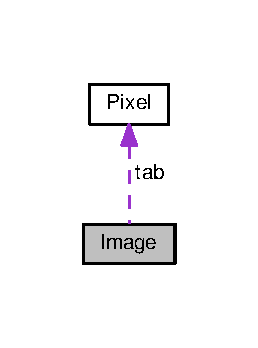
\includegraphics[width=124pt]{structImage__coll__graph}
\end{center}
\end{figure}
\subsection*{Data Fields}
\begin{DoxyCompactItemize}
\item 
\hyperlink{structPixel}{Pixel} $\ast$$\ast$ \hyperlink{structImage_aad00390430c4e4e3a5a71bb919a4076c}{tab}
\item 
int \hyperlink{structImage_a1fbf685f50372de48b7290cd02a77b0c}{dimx}
\item 
int \hyperlink{structImage_a2e937e4780121e32bce2ccae87069b68}{dimy}
\end{DoxyCompactItemize}


\subsection{Detailed Description}


Definition at line 13 of file Image.\+h.



\subsection{Field Documentation}
\hypertarget{structImage_a1fbf685f50372de48b7290cd02a77b0c}{}\index{Image@{Image}!dimx@{dimx}}
\index{dimx@{dimx}!Image@{Image}}
\subsubsection[{dimx}]{\setlength{\rightskip}{0pt plus 5cm}int Image\+::dimx}\label{structImage_a1fbf685f50372de48b7290cd02a77b0c}


Definition at line 16 of file Image.\+h.

\hypertarget{structImage_a2e937e4780121e32bce2ccae87069b68}{}\index{Image@{Image}!dimy@{dimy}}
\index{dimy@{dimy}!Image@{Image}}
\subsubsection[{dimy}]{\setlength{\rightskip}{0pt plus 5cm}int Image\+::dimy}\label{structImage_a2e937e4780121e32bce2ccae87069b68}


Definition at line 16 of file Image.\+h.

\hypertarget{structImage_aad00390430c4e4e3a5a71bb919a4076c}{}\index{Image@{Image}!tab@{tab}}
\index{tab@{tab}!Image@{Image}}
\subsubsection[{tab}]{\setlength{\rightskip}{0pt plus 5cm}{\bf Pixel}$\ast$$\ast$ Image\+::tab}\label{structImage_aad00390430c4e4e3a5a71bb919a4076c}


Definition at line 15 of file Image.\+h.



The documentation for this struct was generated from the following file\+:\begin{DoxyCompactItemize}
\item 
/home/wadi2a/\+Desktop/11512099/src/\hyperlink{Image_8h}{Image.\+h}\end{DoxyCompactItemize}

\hypertarget{structPixel}{}\section{Pixel Struct Reference}
\label{structPixel}\index{Pixel@{Pixel}}


{\ttfamily \#include $<$Pixel.\+h$>$}

\subsection*{Data Fields}
\begin{DoxyCompactItemize}
\item 
unsigned char \hyperlink{structPixel_a038ad5b3349e7548d17c5d3bec511b94}{r}
\item 
unsigned char \hyperlink{structPixel_a8407845aacf1663d9463475619911686}{g}
\item 
unsigned char \hyperlink{structPixel_a760bdf29b15433d257f119239fcff4d4}{b}
\end{DoxyCompactItemize}


\subsection{Detailed Description}


Definition at line 13 of file Pixel.\+h.



\subsection{Field Documentation}
\hypertarget{structPixel_a760bdf29b15433d257f119239fcff4d4}{}\index{Pixel@{Pixel}!b@{b}}
\index{b@{b}!Pixel@{Pixel}}
\subsubsection[{b}]{\setlength{\rightskip}{0pt plus 5cm}unsigned char Pixel\+::b}\label{structPixel_a760bdf29b15433d257f119239fcff4d4}


Definition at line 15 of file Pixel.\+h.

\hypertarget{structPixel_a8407845aacf1663d9463475619911686}{}\index{Pixel@{Pixel}!g@{g}}
\index{g@{g}!Pixel@{Pixel}}
\subsubsection[{g}]{\setlength{\rightskip}{0pt plus 5cm}unsigned char Pixel\+::g}\label{structPixel_a8407845aacf1663d9463475619911686}


Definition at line 15 of file Pixel.\+h.

\hypertarget{structPixel_a038ad5b3349e7548d17c5d3bec511b94}{}\index{Pixel@{Pixel}!r@{r}}
\index{r@{r}!Pixel@{Pixel}}
\subsubsection[{r}]{\setlength{\rightskip}{0pt plus 5cm}unsigned char Pixel\+::r}\label{structPixel_a038ad5b3349e7548d17c5d3bec511b94}


Definition at line 15 of file Pixel.\+h.



The documentation for this struct was generated from the following file\+:\begin{DoxyCompactItemize}
\item 
/home/wadi2a/\+Desktop/11512099/src/\hyperlink{Pixel_8h}{Pixel.\+h}\end{DoxyCompactItemize}

\chapter{File Documentation}
\hypertarget{Image_8c}{}\section{/home/wadi2a/\+Desktop/11512099/src/\+Image.c File Reference}
\label{Image_8c}\index{/home/wadi2a/\+Desktop/11512099/src/\+Image.\+c@{/home/wadi2a/\+Desktop/11512099/src/\+Image.\+c}}


Fichier .c du Module \hyperlink{structImage}{Image} Fichier qui comporte tout la définition des fonction de ce module.  


{\ttfamily \#include $<$stdio.\+h$>$}\\*
{\ttfamily \#include $<$stdlib.\+h$>$}\\*
{\ttfamily \#include $<$assert.\+h$>$}\\*
{\ttfamily \#include \char`\"{}Image.\+h\char`\"{}}\\*
Include dependency graph for Image.\+c\+:\nopagebreak
\begin{figure}[H]
\begin{center}
\leavevmode
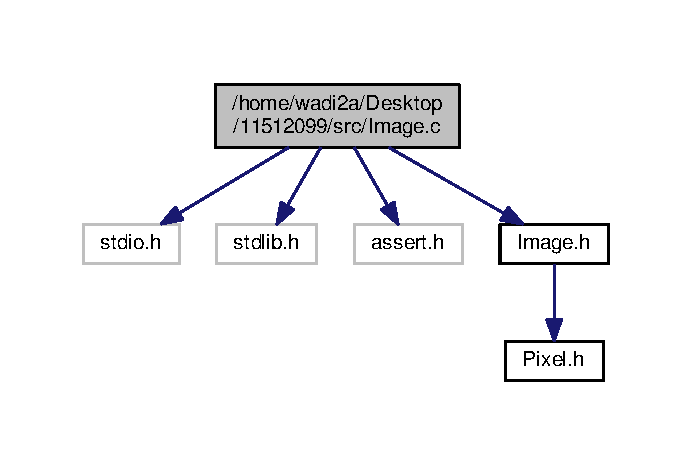
\includegraphics[width=332pt]{Image_8c__incl}
\end{center}
\end{figure}
\subsection*{Functions}
\begin{DoxyCompactItemize}
\item 
void \hyperlink{Image_8c_a6edbdf3bfe3beb4e44246a6c7985055c}{im\+Init} (\hyperlink{structImage}{Image} $\ast$im, const int dimx, const int dimy)
\begin{DoxyCompactList}\small\item\em im\+Init initialise dimx et dimy (après vérification) de la structure \hyperlink{structImage}{Image} puis alloue le tableau de pixel dans le tas \end{DoxyCompactList}\item 
void \hyperlink{Image_8c_a5931290abc22d365ae351381c594613f}{im\+Libere} (\hyperlink{structImage}{Image} $\ast$im)
\begin{DoxyCompactList}\small\item\em im\+Libere Libère la mémoire du tableau de pixels et met les champs dimx et dimy de la structure à 0 \end{DoxyCompactList}\item 
\hyperlink{structImage}{Image} $\ast$ \hyperlink{Image_8c_acd1b5e5f7a7fa80087a1e53bfa4da49d}{im\+Creer} (const int dimx, const int dimy)
\begin{DoxyCompactList}\small\item\em im\+Creer alloue dans le tas une structure \hyperlink{structImage}{Image} puis l\textquotesingle{}initialise avec im\+Init avant de la retourner \end{DoxyCompactList}\item 
void \hyperlink{Image_8c_acf3867531d803daad076cf18d2a14935}{im\+Detruire} (\hyperlink{structImage}{Image} $\ast$pim)
\begin{DoxyCompactList}\small\item\em im\+Detruire Libere le tableau de pixel en appelant im\+Libere puis détruit la structure image \end{DoxyCompactList}\item 
\hyperlink{structPixel}{Pixel} \hyperlink{Image_8c_a1cb04a46ed83be9a0c49b3b884c91d62}{get\+Pix} (const \hyperlink{structImage}{Image} $\ast$im, const int x, const int y)
\begin{DoxyCompactList}\small\item\em get\+Pix récupère le pixel de coordonnées (x,y) en vérifiant leur validité \end{DoxyCompactList}\item 
void \hyperlink{Image_8c_a7da553849b645f075994622df5bca888}{set\+Pix} (\hyperlink{structImage}{Image} $\ast$im, const int x, const int y, \hyperlink{structPixel}{Pixel} couleur)
\begin{DoxyCompactList}\small\item\em set\+Pix modifie le pixel de coordonnées (x,y) \end{DoxyCompactList}\item 
void \hyperlink{Image_8c_a01084dc5c10d366999aece5432dc823f}{im\+Dessine\+Rectangle} (\hyperlink{structImage}{Image} $\ast$im, const int Xmin, const int Ymin, const int Xmax, const int Ymax, \hyperlink{structPixel}{Pixel} couleur)
\begin{DoxyCompactList}\small\item\em im\+Dessine\+Rectangle dessine un rectangle de couleur dans l\textquotesingle{}image en utilisant set\+Pix \end{DoxyCompactList}\item 
void \hyperlink{Image_8c_ae11c1ca640aae91cb1419158ad5bdf59}{im\+Effacer} (\hyperlink{structImage}{Image} $\ast$im, const \hyperlink{structPixel}{Pixel} couleur)
\begin{DoxyCompactList}\small\item\em im\+Effacer efface l\textquotesingle{}image en appelant im\+Dessine\+Rectangle avec le bon rectangle \end{DoxyCompactList}\item 
void \hyperlink{Image_8c_a20b9ad35b6db7bd09d7452574d04dd50}{im\+Sauver} (const \hyperlink{structImage}{Image} $\ast$p\+Im, const char filename\mbox{[}$\,$\mbox{]})
\begin{DoxyCompactList}\small\item\em im\+Sauver Enregistre l\textquotesingle{}image \end{DoxyCompactList}\item 
void \hyperlink{Image_8c_a0a1f0b9be4b910e1cfc2648cfa9e38fd}{im\+Ouvrir} (\hyperlink{structImage}{Image} $\ast$p\+Im, const char filename\mbox{[}$\,$\mbox{]})
\begin{DoxyCompactList}\small\item\em im\+Ouvrir ouvre l\textquotesingle{}image \end{DoxyCompactList}\item 
void \hyperlink{Image_8c_afadf8ab43119d304c72e201d0d95164d}{im\+Printf} (const \hyperlink{structImage}{Image} $\ast$p\+Im)
\begin{DoxyCompactList}\small\item\em im\+Printf affiche le contenue de chaque pixel dans l\textquotesingle{}image \end{DoxyCompactList}\item 
void \hyperlink{Image_8c_a8d4964490fb1a67b590ce77acd78031f}{im\+Test\+Regression} ()
\begin{DoxyCompactList}\small\item\em im\+Test\+Regression Effectue une série de tests vérifiant que le module fonctionne et que les champs de la structure sont conformes \end{DoxyCompactList}\end{DoxyCompactItemize}


\subsection{Detailed Description}
Fichier .c du Module \hyperlink{structImage}{Image} Fichier qui comporte tout la définition des fonction de ce module. 

\begin{DoxyAuthor}{Author}
B\+E\+N A\+I\+S\+S\+A O\+U\+A\+D\+I\+E
\end{DoxyAuthor}
\begin{DoxyVersion}{Version}
1.\+0 
\end{DoxyVersion}
\begin{DoxyDate}{Date}
2016/02/10 
\end{DoxyDate}


\subsection{Function Documentation}
\hypertarget{Image_8c_a1cb04a46ed83be9a0c49b3b884c91d62}{}\index{Image.\+c@{Image.\+c}!get\+Pix@{get\+Pix}}
\index{get\+Pix@{get\+Pix}!Image.\+c@{Image.\+c}}
\subsubsection[{get\+Pix}]{\setlength{\rightskip}{0pt plus 5cm}{\bf Pixel} get\+Pix (
\begin{DoxyParamCaption}
\item[{const {\bf Image} $\ast$}]{im, }
\item[{const int}]{x, }
\item[{const int}]{y}
\end{DoxyParamCaption}
)}\label{Image_8c_a1cb04a46ed83be9a0c49b3b884c91d62}


get\+Pix récupère le pixel de coordonnées (x,y) en vérifiant leur validité 


\begin{DoxyParams}[1]{Parameters}
\mbox{\tt in,out}  & {\em im} & la structure image \\
\hline
\mbox{\tt in}  & {\em x} & Entier qui désigne les cordonnée de l\textquotesingle{}image sur l\textquotesingle{}axe des x \\
\hline
\mbox{\tt in}  & {\em y} & Entier qui désigne les cordonnée de l\textquotesingle{}image sur l\textquotesingle{}axe des y \\
\hline
\end{DoxyParams}
\begin{DoxyReturn}{Returns}
lien vers une pixel.
\end{DoxyReturn}

\begin{DoxyCode}
1 getPix(&im,200,352);
\end{DoxyCode}
 \begin{DoxyWarning}{Warning}
x et y doivent etre inclu dans l\textquotesingle{}intervalle des dimensions 
\end{DoxyWarning}


Definition at line 55 of file Image.\+c.


\begin{DoxyCode}
56 \{
57 
58     assert(x<im->dimx && y<im->dimy);
59     \textcolor{keywordflow}{return} im->\hyperlink{structImage_aad00390430c4e4e3a5a71bb919a4076c}{tab}[x][y];
60 
61 \}
\end{DoxyCode}


Here is the caller graph for this function\+:\nopagebreak
\begin{figure}[H]
\begin{center}
\leavevmode
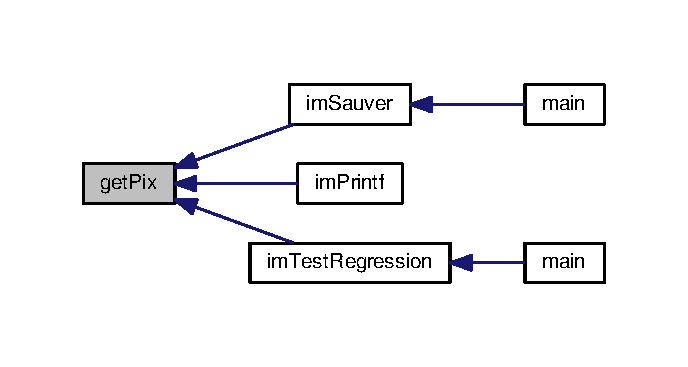
\includegraphics[width=330pt]{Image_8c_a1cb04a46ed83be9a0c49b3b884c91d62_icgraph}
\end{center}
\end{figure}


\hypertarget{Image_8c_acd1b5e5f7a7fa80087a1e53bfa4da49d}{}\index{Image.\+c@{Image.\+c}!im\+Creer@{im\+Creer}}
\index{im\+Creer@{im\+Creer}!Image.\+c@{Image.\+c}}
\subsubsection[{im\+Creer}]{\setlength{\rightskip}{0pt plus 5cm}{\bf Image}$\ast$ im\+Creer (
\begin{DoxyParamCaption}
\item[{const int}]{dimx, }
\item[{const int}]{dimy}
\end{DoxyParamCaption}
)}\label{Image_8c_acd1b5e5f7a7fa80087a1e53bfa4da49d}


im\+Creer alloue dans le tas une structure \hyperlink{structImage}{Image} puis l\textquotesingle{}initialise avec im\+Init avant de la retourner 


\begin{DoxyParams}[1]{Parameters}
\mbox{\tt in}  & {\em dimx} & Entier qui désigne la largeur de l\textquotesingle{}image. \\
\hline
\mbox{\tt in}  & {\em dimy} & Entier qui désigne la hauteur de l\textquotesingle{}image. \\
\hline
\end{DoxyParams}
\begin{DoxyReturn}{Returns}
lien sur image. 
\begin{DoxyCode}
1 imCreer(500,500);
\end{DoxyCode}
 
\end{DoxyReturn}
\begin{DoxyWarning}{Warning}
les dimension de l\textquotesingle{}image doivent etre dimx$>$0 et dimy$>$0 
\end{DoxyWarning}


Definition at line 40 of file Image.\+c.


\begin{DoxyCode}
41 \{
42     \hyperlink{structImage}{Image} * im=malloc( \textcolor{keyword}{sizeof}(\hyperlink{structImage}{Image}));
43 
44     \hyperlink{Image_8c_a6edbdf3bfe3beb4e44246a6c7985055c}{imInit}(im,dimx,dimy);
45     \textcolor{keywordflow}{return} im;
46 \}
\end{DoxyCode}


Here is the call graph for this function\+:\nopagebreak
\begin{figure}[H]
\begin{center}
\leavevmode
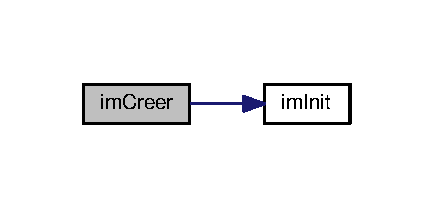
\includegraphics[width=208pt]{Image_8c_acd1b5e5f7a7fa80087a1e53bfa4da49d_cgraph}
\end{center}
\end{figure}




Here is the caller graph for this function\+:\nopagebreak
\begin{figure}[H]
\begin{center}
\leavevmode
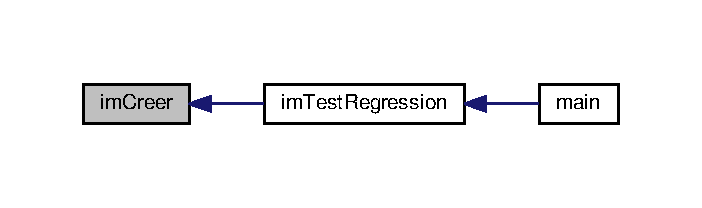
\includegraphics[width=337pt]{Image_8c_acd1b5e5f7a7fa80087a1e53bfa4da49d_icgraph}
\end{center}
\end{figure}


\hypertarget{Image_8c_a01084dc5c10d366999aece5432dc823f}{}\index{Image.\+c@{Image.\+c}!im\+Dessine\+Rectangle@{im\+Dessine\+Rectangle}}
\index{im\+Dessine\+Rectangle@{im\+Dessine\+Rectangle}!Image.\+c@{Image.\+c}}
\subsubsection[{im\+Dessine\+Rectangle}]{\setlength{\rightskip}{0pt plus 5cm}void im\+Dessine\+Rectangle (
\begin{DoxyParamCaption}
\item[{{\bf Image} $\ast$}]{im, }
\item[{const int}]{Xmin, }
\item[{const int}]{Ymin, }
\item[{const int}]{Xmax, }
\item[{const int}]{Ymax, }
\item[{const {\bf Pixel}}]{couleur}
\end{DoxyParamCaption}
)}\label{Image_8c_a01084dc5c10d366999aece5432dc823f}


im\+Dessine\+Rectangle dessine un rectangle de couleur dans l\textquotesingle{}image en utilisant set\+Pix 


\begin{DoxyParams}[1]{Parameters}
\mbox{\tt in,out}  & {\em im} & la structure image \\
\hline
\mbox{\tt in}  & {\em Xmin} & Entier qui désigne le début du rectangle sur l\textquotesingle{}axe des x \\
\hline
\mbox{\tt in}  & {\em Xmax} & Entier qui désigne la fin du rectangle sur l\textquotesingle{}axe des x \\
\hline
\mbox{\tt in}  & {\em Ymin} & Entier qui désigne le début du rectangle sur l\textquotesingle{}axe des y \\
\hline
\mbox{\tt in}  & {\em Ymax} & Entier qui désigne la fin du rectangle sur l\textquotesingle{}axe des x \\
\hline
\mbox{\tt in}  & {\em couleur} & \hyperlink{structPixel}{Pixel} qui contient les valeurs du couleurs que nous allons l\textquotesingle{}affecté au triangle \\
\hline
\end{DoxyParams}
\begin{DoxyReturn}{Returns}
none.
\end{DoxyReturn}

\begin{DoxyCode}
1 imDessineRectangle(&im,100,100,200,352,couleur);
\end{DoxyCode}
 \begin{DoxyWarning}{Warning}
Xmin,Xmax,Ymin,Ymax doivent etre inclu dans l\textquotesingle{}intervalle des dimensions 
\end{DoxyWarning}


Definition at line 72 of file Image.\+c.


\begin{DoxyCode}
73 \{   \textcolor{keywordtype}{int} i=0,j=0;
74     assert((Xmin>=0) && (Xmax<im->dimx) && (Ymin>=0) && (Ymax<im->dimy));
75     \textcolor{comment}{/*}
76 \textcolor{comment}{    pour dessiner un triangle vide a l'interieur}
77 \textcolor{comment}{    for(i=Xmin;i<=Xmax;i++) setPix(im,i,Ymin,couleur);}
78 \textcolor{comment}{    for(i=Ymin;i<=Ymax;i++) setPix(im,Xmin,i,couleur);}
79 \textcolor{comment}{    for(i=Xmin;i<=Xmax;i++) setPix(im,i,Ymax,couleur);}
80 \textcolor{comment}{    for(i=Ymin;i<=Ymax;i++) setPix(im,Xmax,i,couleur);*/}
81     \textcolor{keywordflow}{for}(i=Xmin;i<=Xmax;i++)
82     \{
83         \textcolor{keywordflow}{for}(j=Ymin;j<=Ymax;j++)
84         \{
85             \hyperlink{Image_8c_a7da553849b645f075994622df5bca888}{setPix}(im,i,j,couleur);
86         \}
87     \}
88 \}
\end{DoxyCode}


Here is the call graph for this function\+:\nopagebreak
\begin{figure}[H]
\begin{center}
\leavevmode
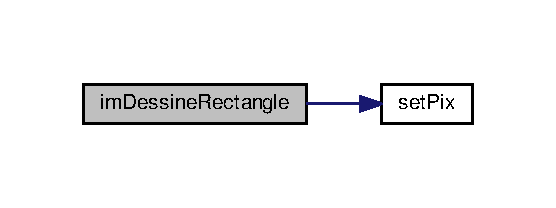
\includegraphics[width=267pt]{Image_8c_a01084dc5c10d366999aece5432dc823f_cgraph}
\end{center}
\end{figure}




Here is the caller graph for this function\+:\nopagebreak
\begin{figure}[H]
\begin{center}
\leavevmode
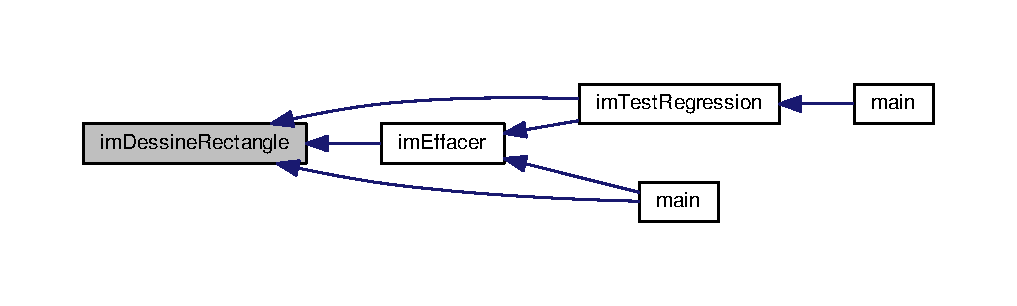
\includegraphics[width=350pt]{Image_8c_a01084dc5c10d366999aece5432dc823f_icgraph}
\end{center}
\end{figure}


\hypertarget{Image_8c_acf3867531d803daad076cf18d2a14935}{}\index{Image.\+c@{Image.\+c}!im\+Detruire@{im\+Detruire}}
\index{im\+Detruire@{im\+Detruire}!Image.\+c@{Image.\+c}}
\subsubsection[{im\+Detruire}]{\setlength{\rightskip}{0pt plus 5cm}void im\+Detruire (
\begin{DoxyParamCaption}
\item[{{\bf Image} $\ast$}]{pim}
\end{DoxyParamCaption}
)}\label{Image_8c_acf3867531d803daad076cf18d2a14935}


im\+Detruire Libere le tableau de pixel en appelant im\+Libere puis détruit la structure image 


\begin{DoxyParams}[1]{Parameters}
\mbox{\tt in,out}  & {\em im} & la structure image à détruire. \\
\hline
\end{DoxyParams}
\begin{DoxyReturn}{Returns}
none. 
\begin{DoxyCode}
1 imDetruire(Image *pim);
\end{DoxyCode}
 
\end{DoxyReturn}


Definition at line 48 of file Image.\+c.


\begin{DoxyCode}
49 \{
50     \hyperlink{Image_8c_a5931290abc22d365ae351381c594613f}{imLibere}(pim);
51     free(pim);
52 
53 
54 \}
\end{DoxyCode}


Here is the call graph for this function\+:\nopagebreak
\begin{figure}[H]
\begin{center}
\leavevmode
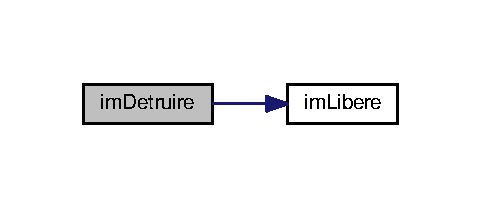
\includegraphics[width=231pt]{Image_8c_acf3867531d803daad076cf18d2a14935_cgraph}
\end{center}
\end{figure}




Here is the caller graph for this function\+:\nopagebreak
\begin{figure}[H]
\begin{center}
\leavevmode
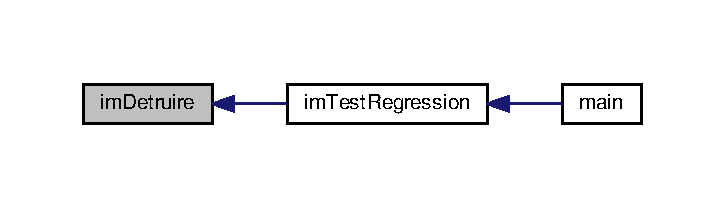
\includegraphics[width=348pt]{Image_8c_acf3867531d803daad076cf18d2a14935_icgraph}
\end{center}
\end{figure}


\hypertarget{Image_8c_ae11c1ca640aae91cb1419158ad5bdf59}{}\index{Image.\+c@{Image.\+c}!im\+Effacer@{im\+Effacer}}
\index{im\+Effacer@{im\+Effacer}!Image.\+c@{Image.\+c}}
\subsubsection[{im\+Effacer}]{\setlength{\rightskip}{0pt plus 5cm}void im\+Effacer (
\begin{DoxyParamCaption}
\item[{{\bf Image} $\ast$}]{im, }
\item[{const {\bf Pixel}}]{couleur}
\end{DoxyParamCaption}
)}\label{Image_8c_ae11c1ca640aae91cb1419158ad5bdf59}


im\+Effacer efface l\textquotesingle{}image en appelant im\+Dessine\+Rectangle avec le bon rectangle 


\begin{DoxyParams}[1]{Parameters}
\mbox{\tt in,out}  & {\em im} & la structure image \\
\hline
\mbox{\tt in}  & {\em couleur} & \hyperlink{structPixel}{Pixel} qui contient les valeurs du couleurs que nous allons l\textquotesingle{}affecté au triangle \\
\hline
\end{DoxyParams}
\begin{DoxyReturn}{Returns}
none.
\end{DoxyReturn}

\begin{DoxyCode}
1 imEffacer(&im,couleur);
\end{DoxyCode}
 

Definition at line 89 of file Image.\+c.


\begin{DoxyCode}
90 \{
91 
92     \hyperlink{Image_8c_a01084dc5c10d366999aece5432dc823f}{imDessineRectangle}(im,0,0,im->\hyperlink{structImage_a1fbf685f50372de48b7290cd02a77b0c}{dimx}-1,im->\hyperlink{structImage_a2e937e4780121e32bce2ccae87069b68}{dimy}-1,couleur);
93 
94 \}
\end{DoxyCode}


Here is the call graph for this function\+:\nopagebreak
\begin{figure}[H]
\begin{center}
\leavevmode
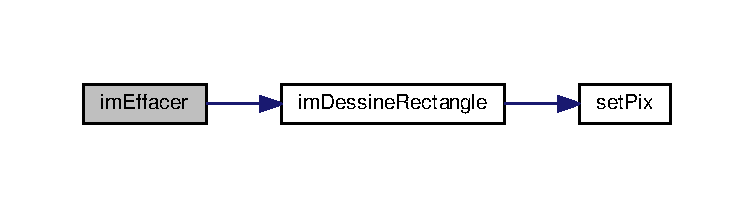
\includegraphics[width=350pt]{Image_8c_ae11c1ca640aae91cb1419158ad5bdf59_cgraph}
\end{center}
\end{figure}




Here is the caller graph for this function\+:\nopagebreak
\begin{figure}[H]
\begin{center}
\leavevmode
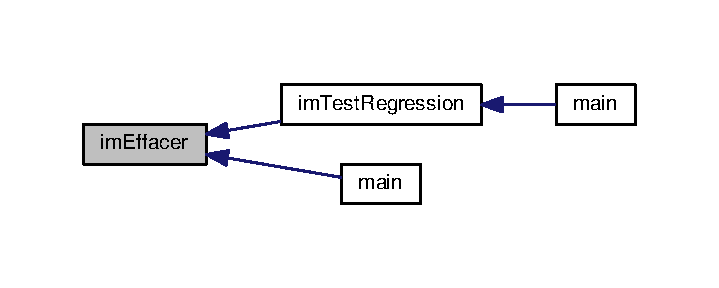
\includegraphics[width=345pt]{Image_8c_ae11c1ca640aae91cb1419158ad5bdf59_icgraph}
\end{center}
\end{figure}


\hypertarget{Image_8c_a6edbdf3bfe3beb4e44246a6c7985055c}{}\index{Image.\+c@{Image.\+c}!im\+Init@{im\+Init}}
\index{im\+Init@{im\+Init}!Image.\+c@{Image.\+c}}
\subsubsection[{im\+Init}]{\setlength{\rightskip}{0pt plus 5cm}void im\+Init (
\begin{DoxyParamCaption}
\item[{{\bf Image} $\ast$}]{im, }
\item[{const int}]{dimx, }
\item[{const int}]{dimy}
\end{DoxyParamCaption}
)}\label{Image_8c_a6edbdf3bfe3beb4e44246a6c7985055c}


im\+Init initialise dimx et dimy (après vérification) de la structure \hyperlink{structImage}{Image} puis alloue le tableau de pixel dans le tas 


\begin{DoxyParams}[1]{Parameters}
\mbox{\tt in,out}  & {\em im} & la structure image à initialisé \\
\hline
\mbox{\tt in}  & {\em dimx} & Entier qui désigne la largeur de l\textquotesingle{}image \\
\hline
\mbox{\tt in}  & {\em dimy} & Entier qui désigne la hauteur de l\textquotesingle{}image \\
\hline
\end{DoxyParams}
\begin{DoxyReturn}{Returns}
none.
\end{DoxyReturn}

\begin{DoxyCode}
1 imInit(&im,500,500);
\end{DoxyCode}
 \begin{DoxyWarning}{Warning}
les dimension de l\textquotesingle{}image doivent etre dimx$>$0 et dimy$>$0 
\end{DoxyWarning}


Definition at line 15 of file Image.\+c.


\begin{DoxyCode}
16 \{
17     \textcolor{keywordtype}{int} i;
18 
19     assert(dimx>0 && dimy>0);
20     im->\hyperlink{structImage_aad00390430c4e4e3a5a71bb919a4076c}{tab}=malloc(dimy * \textcolor{keyword}{sizeof}(\hyperlink{structPixel}{Pixel}*));
21     \textcolor{keywordflow}{for}(i=0;i<dimy;i++)
22     \{
23         im->\hyperlink{structImage_aad00390430c4e4e3a5a71bb919a4076c}{tab}[i]=(\hyperlink{structPixel}{Pixel}*)malloc(dimy*\textcolor{keyword}{sizeof}(\hyperlink{structPixel}{Pixel}));
24     \}
25     im->\hyperlink{structImage_a1fbf685f50372de48b7290cd02a77b0c}{dimx}=dimx;
26     im->\hyperlink{structImage_a2e937e4780121e32bce2ccae87069b68}{dimy}=dimy;
27  
28 \}
\end{DoxyCode}


Here is the caller graph for this function\+:\nopagebreak
\begin{figure}[H]
\begin{center}
\leavevmode
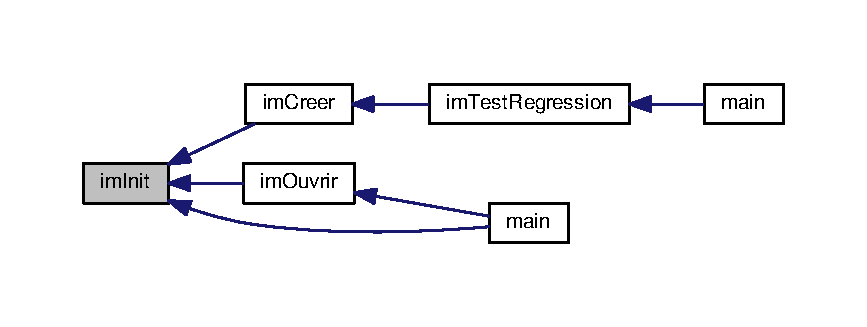
\includegraphics[width=350pt]{Image_8c_a6edbdf3bfe3beb4e44246a6c7985055c_icgraph}
\end{center}
\end{figure}


\hypertarget{Image_8c_a5931290abc22d365ae351381c594613f}{}\index{Image.\+c@{Image.\+c}!im\+Libere@{im\+Libere}}
\index{im\+Libere@{im\+Libere}!Image.\+c@{Image.\+c}}
\subsubsection[{im\+Libere}]{\setlength{\rightskip}{0pt plus 5cm}void im\+Libere (
\begin{DoxyParamCaption}
\item[{{\bf Image} $\ast$}]{im}
\end{DoxyParamCaption}
)}\label{Image_8c_a5931290abc22d365ae351381c594613f}


im\+Libere Libère la mémoire du tableau de pixels et met les champs dimx et dimy de la structure à 0 


\begin{DoxyParams}[1]{Parameters}
\mbox{\tt in,out}  & {\em im} & la structure image à initialisé. \\
\hline
\end{DoxyParams}
\begin{DoxyReturn}{Returns}
none. 
\begin{DoxyCode}
1 void imLibere(&im);
\end{DoxyCode}
 
\end{DoxyReturn}


Definition at line 30 of file Image.\+c.


\begin{DoxyCode}
31 \{   \textcolor{keywordtype}{int} i;
32     \textcolor{keywordflow}{for}(i=0;i<im->\hyperlink{structImage_a2e937e4780121e32bce2ccae87069b68}{dimy};i++)
33     \{
34         free(im->\hyperlink{structImage_aad00390430c4e4e3a5a71bb919a4076c}{tab}[i]);
35     \}
36 
37     im->\hyperlink{structImage_a1fbf685f50372de48b7290cd02a77b0c}{dimx}=0;
38     im->\hyperlink{structImage_a2e937e4780121e32bce2ccae87069b68}{dimy}=0;
39 \}
\end{DoxyCode}


Here is the caller graph for this function\+:\nopagebreak
\begin{figure}[H]
\begin{center}
\leavevmode
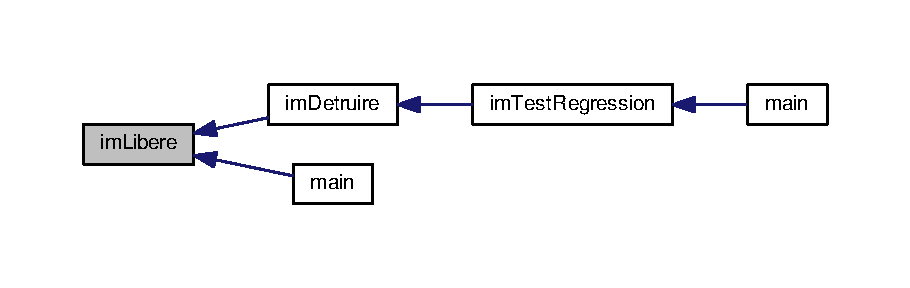
\includegraphics[width=350pt]{Image_8c_a5931290abc22d365ae351381c594613f_icgraph}
\end{center}
\end{figure}


\hypertarget{Image_8c_a0a1f0b9be4b910e1cfc2648cfa9e38fd}{}\index{Image.\+c@{Image.\+c}!im\+Ouvrir@{im\+Ouvrir}}
\index{im\+Ouvrir@{im\+Ouvrir}!Image.\+c@{Image.\+c}}
\subsubsection[{im\+Ouvrir}]{\setlength{\rightskip}{0pt plus 5cm}void im\+Ouvrir (
\begin{DoxyParamCaption}
\item[{{\bf Image} $\ast$}]{p\+Im, }
\item[{const char}]{filename\mbox{[}$\,$\mbox{]}}
\end{DoxyParamCaption}
)}\label{Image_8c_a0a1f0b9be4b910e1cfc2648cfa9e38fd}


im\+Ouvrir ouvre l\textquotesingle{}image 


\begin{DoxyParams}[1]{Parameters}
\mbox{\tt in,out}  & {\em im} & la structure image \\
\hline
\mbox{\tt in}  & {\em chaine} & de caractère qui désigne l\textquotesingle{}emplacement de l\textquotesingle{}image \\
\hline
\end{DoxyParams}
\begin{DoxyReturn}{Returns}
none.
\end{DoxyReturn}

\begin{DoxyCode}
1 imOuvrir(&im,"./data/toto.ppm");
\end{DoxyCode}
 \begin{DoxyWarning}{Warning}
l\textquotesingle{}image doit etre crée avant l\textquotesingle{}execution de cette procedure 
\end{DoxyWarning}


Definition at line 118 of file Image.\+c.


\begin{DoxyCode}
118                                                  \{
119     FILE* f;
120     \hyperlink{structPixel}{Pixel} pix;
121     \textcolor{keywordtype}{int} x, y, dimx, dimy;
122 
123     f = fopen(filename, \textcolor{stringliteral}{"r"});
124     \textcolor{keywordflow}{if} (f==NULL) \{
125         printf(\textcolor{stringliteral}{"Erreur lors de l'ouverture de %s\(\backslash\)n"}, filename);
126         assert( f );
127     \}
128 
129     assert( fscanf( f , \textcolor{stringliteral}{"P3\(\backslash\)n%d %d\(\backslash\)n255\(\backslash\)n"}, &dimx, &dimy) == 2 );
130     \hyperlink{Image_8c_a6edbdf3bfe3beb4e44246a6c7985055c}{imInit}( pIm, dimx, dimy);
131 
132     \textcolor{keywordflow}{for}(y=0;y<pIm->\hyperlink{structImage_a2e937e4780121e32bce2ccae87069b68}{dimy};++y)
133         \textcolor{keywordflow}{for}(x=0;x<pIm->\hyperlink{structImage_a1fbf685f50372de48b7290cd02a77b0c}{dimx};++x) \{
134             assert( fscanf(f, \textcolor{stringliteral}{"%c %c %c  "}, &pix.\hyperlink{structPixel_a038ad5b3349e7548d17c5d3bec511b94}{r}, &pix.\hyperlink{structPixel_a8407845aacf1663d9463475619911686}{g}, &pix.\hyperlink{structPixel_a760bdf29b15433d257f119239fcff4d4}{b}) == 3 );
135             \hyperlink{Image_8c_a7da553849b645f075994622df5bca888}{setPix}(pIm,x,y,pix);
136         \}
137     fclose(f);
138     printf(\textcolor{stringliteral}{"Lecture de l'image %s ...OK\(\backslash\)n"}, filename);
139 \}
\end{DoxyCode}


Here is the call graph for this function\+:\nopagebreak
\begin{figure}[H]
\begin{center}
\leavevmode
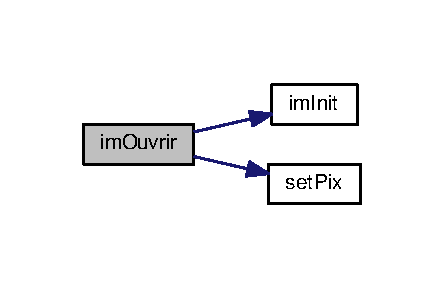
\includegraphics[width=213pt]{Image_8c_a0a1f0b9be4b910e1cfc2648cfa9e38fd_cgraph}
\end{center}
\end{figure}




Here is the caller graph for this function\+:\nopagebreak
\begin{figure}[H]
\begin{center}
\leavevmode
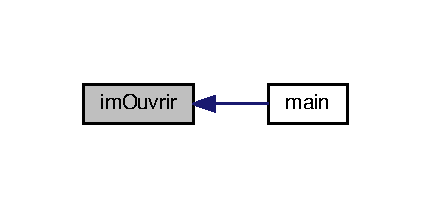
\includegraphics[width=207pt]{Image_8c_a0a1f0b9be4b910e1cfc2648cfa9e38fd_icgraph}
\end{center}
\end{figure}


\hypertarget{Image_8c_afadf8ab43119d304c72e201d0d95164d}{}\index{Image.\+c@{Image.\+c}!im\+Printf@{im\+Printf}}
\index{im\+Printf@{im\+Printf}!Image.\+c@{Image.\+c}}
\subsubsection[{im\+Printf}]{\setlength{\rightskip}{0pt plus 5cm}void im\+Printf (
\begin{DoxyParamCaption}
\item[{const {\bf Image} $\ast$}]{p\+Im}
\end{DoxyParamCaption}
)}\label{Image_8c_afadf8ab43119d304c72e201d0d95164d}


im\+Printf affiche le contenue de chaque pixel dans l\textquotesingle{}image 


\begin{DoxyParams}[1]{Parameters}
\mbox{\tt in,out}  & {\em im} & la structure image \\
\hline
\end{DoxyParams}
\begin{DoxyReturn}{Returns}
none.
\end{DoxyReturn}

\begin{DoxyCode}
1 imPrintf(&im);
\end{DoxyCode}
 \begin{DoxyWarning}{Warning}
l\textquotesingle{}image doit etre crée avant l\textquotesingle{}execution de cette procedure 
\end{DoxyWarning}


Definition at line 141 of file Image.\+c.


\begin{DoxyCode}
141                                 \{
142     \textcolor{keywordtype}{int} x,y;
143     \hyperlink{structPixel}{Pixel} pix;
144 
145     printf( \textcolor{stringliteral}{"%d %d\(\backslash\)n"}, pIm->\hyperlink{structImage_a1fbf685f50372de48b7290cd02a77b0c}{dimx}, pIm->\hyperlink{structImage_a2e937e4780121e32bce2ccae87069b68}{dimy});      \textcolor{comment}{/* dimension de l'image*/}
146 
147     \textcolor{keywordflow}{for}(y=0;y<pIm->\hyperlink{structImage_a2e937e4780121e32bce2ccae87069b68}{dimy};++y) \{
148         \textcolor{keywordflow}{for}(x=0;x<pIm->\hyperlink{structImage_a1fbf685f50372de48b7290cd02a77b0c}{dimx};++x) \{
149             pix = \hyperlink{Image_8c_a1cb04a46ed83be9a0c49b3b884c91d62}{getPix}(pIm,x,y);
150             printf(\textcolor{stringliteral}{"%d %d %d  "}, pix.\hyperlink{structPixel_a038ad5b3349e7548d17c5d3bec511b94}{r}, pix.\hyperlink{structPixel_a8407845aacf1663d9463475619911686}{g}, pix.\hyperlink{structPixel_a760bdf29b15433d257f119239fcff4d4}{b});
151         \}
152         printf(\textcolor{stringliteral}{"\(\backslash\)n"});
153     \}
154 \}
\end{DoxyCode}


Here is the call graph for this function\+:\nopagebreak
\begin{figure}[H]
\begin{center}
\leavevmode
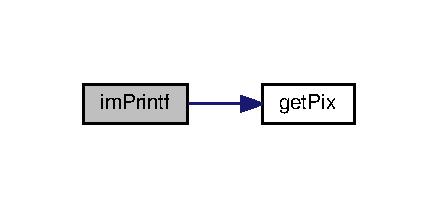
\includegraphics[width=210pt]{Image_8c_afadf8ab43119d304c72e201d0d95164d_cgraph}
\end{center}
\end{figure}


\hypertarget{Image_8c_a20b9ad35b6db7bd09d7452574d04dd50}{}\index{Image.\+c@{Image.\+c}!im\+Sauver@{im\+Sauver}}
\index{im\+Sauver@{im\+Sauver}!Image.\+c@{Image.\+c}}
\subsubsection[{im\+Sauver}]{\setlength{\rightskip}{0pt plus 5cm}void im\+Sauver (
\begin{DoxyParamCaption}
\item[{const {\bf Image} $\ast$}]{p\+Im, }
\item[{const char}]{filename\mbox{[}$\,$\mbox{]}}
\end{DoxyParamCaption}
)}\label{Image_8c_a20b9ad35b6db7bd09d7452574d04dd50}


im\+Sauver Enregistre l\textquotesingle{}image 


\begin{DoxyParams}[1]{Parameters}
\mbox{\tt in,out}  & {\em im} & la structure image \\
\hline
\mbox{\tt in}  & {\em chaine} & de caractère qui désigne l\textquotesingle{}emplacement de l\textquotesingle{}image \\
\hline
\end{DoxyParams}
\begin{DoxyReturn}{Returns}
none.
\end{DoxyReturn}

\begin{DoxyCode}
1 imSauver(&im,"./data/toto.ppm");
\end{DoxyCode}
 \begin{DoxyWarning}{Warning}
l\textquotesingle{}image doit etre crée avant l\textquotesingle{}execution de cette procedure 
\end{DoxyWarning}


Definition at line 96 of file Image.\+c.


\begin{DoxyCode}
96                                                        \{
97     FILE* f;
98     \hyperlink{structPixel}{Pixel} pix;
99     \textcolor{keywordtype}{int} x,y;
100 
101     f = fopen(filename, \textcolor{stringliteral}{"w"});
102     \textcolor{keywordflow}{if} (f==NULL) \{
103         printf(\textcolor{stringliteral}{"Erreur lors de l'ouverture de %s\(\backslash\)n"}, filename);
104         assert( f );
105     \}
106     fprintf( f , \textcolor{stringliteral}{"P3\(\backslash\)n"});                           \textcolor{comment}{/*P3 = ascii avec 3 composantes RGB*/}
107     fprintf( f , \textcolor{stringliteral}{"%d %d\(\backslash\)n"}, pIm->\hyperlink{structImage_a1fbf685f50372de48b7290cd02a77b0c}{dimx}, pIm->\hyperlink{structImage_a2e937e4780121e32bce2ccae87069b68}{dimy});  \textcolor{comment}{/* dimension de l'image*/}
108     fprintf( f , \textcolor{stringliteral}{"255\(\backslash\)n"});                          \textcolor{comment}{/* chaque composante est comprise entre 0 et 255*/}
109 
110     \textcolor{keywordflow}{for}(y=0;y<pIm->\hyperlink{structImage_a2e937e4780121e32bce2ccae87069b68}{dimy};++y)
111         \textcolor{keywordflow}{for}(x=0;x<pIm->\hyperlink{structImage_a1fbf685f50372de48b7290cd02a77b0c}{dimx};++x) \{
112             pix = \hyperlink{Image_8c_a1cb04a46ed83be9a0c49b3b884c91d62}{getPix}(pIm,x++,y);
113             fprintf(f, \textcolor{stringliteral}{"%d %d %d  "}, pix.\hyperlink{structPixel_a038ad5b3349e7548d17c5d3bec511b94}{r}, pix.\hyperlink{structPixel_a8407845aacf1663d9463475619911686}{g}, pix.\hyperlink{structPixel_a760bdf29b15433d257f119239fcff4d4}{b});
114         \}
115     printf(\textcolor{stringliteral}{"Sauvegarde de l'image %s ...OK\(\backslash\)n"}, filename);
116     fclose(f);
117 \}
\end{DoxyCode}


Here is the call graph for this function\+:\nopagebreak
\begin{figure}[H]
\begin{center}
\leavevmode
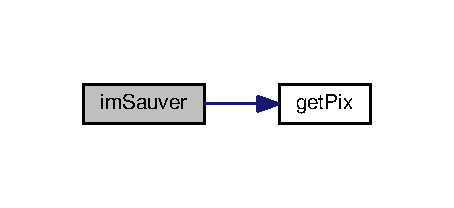
\includegraphics[width=218pt]{Image_8c_a20b9ad35b6db7bd09d7452574d04dd50_cgraph}
\end{center}
\end{figure}




Here is the caller graph for this function\+:\nopagebreak
\begin{figure}[H]
\begin{center}
\leavevmode
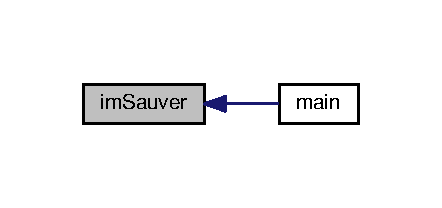
\includegraphics[width=212pt]{Image_8c_a20b9ad35b6db7bd09d7452574d04dd50_icgraph}
\end{center}
\end{figure}


\hypertarget{Image_8c_a8d4964490fb1a67b590ce77acd78031f}{}\index{Image.\+c@{Image.\+c}!im\+Test\+Regression@{im\+Test\+Regression}}
\index{im\+Test\+Regression@{im\+Test\+Regression}!Image.\+c@{Image.\+c}}
\subsubsection[{im\+Test\+Regression}]{\setlength{\rightskip}{0pt plus 5cm}void im\+Test\+Regression (
\begin{DoxyParamCaption}
{}
\end{DoxyParamCaption}
)}\label{Image_8c_a8d4964490fb1a67b590ce77acd78031f}


im\+Test\+Regression Effectue une série de tests vérifiant que le module fonctionne et que les champs de la structure sont conformes 


\begin{DoxyParams}{Parameters}
{\em none} & \\
\hline
\end{DoxyParams}
\begin{DoxyReturn}{Returns}
none.
\end{DoxyReturn}

\begin{DoxyCode}
1 imTestRegression();
\end{DoxyCode}
 

Definition at line 156 of file Image.\+c.


\begin{DoxyCode}
157 \{
158     \hyperlink{structImage}{Image} * im;
159     \textcolor{keywordtype}{int} dimx,dimy;\textcolor{keywordtype}{int} i,j;\hyperlink{structPixel}{Pixel} couleur2 = \{ 0, 0, 0 \};
160     \hyperlink{structPixel}{Pixel} couleur;couleur.\hyperlink{structPixel_a760bdf29b15433d257f119239fcff4d4}{b}=8;couleur.\hyperlink{structPixel_a038ad5b3349e7548d17c5d3bec511b94}{r}=1;couleur.\hyperlink{structPixel_a8407845aacf1663d9463475619911686}{g}=1;
161 
162     printf(\textcolor{stringliteral}{"Donnez la dimension de ton image:\(\backslash\)n dimx:"});
163     scanf(\textcolor{stringliteral}{"%d"},&dimx);
164     printf(\textcolor{stringliteral}{"dimy:"});
165     scanf(\textcolor{stringliteral}{"%d"},&dimy);
166     im=\hyperlink{Image_8c_acd1b5e5f7a7fa80087a1e53bfa4da49d}{imCreer}(dimx,dimy);
167     printf(\textcolor{stringliteral}{"Taille de l'image :%dpx*%dpx"},im->\hyperlink{structImage_a1fbf685f50372de48b7290cd02a77b0c}{dimx},im->\hyperlink{structImage_a2e937e4780121e32bce2ccae87069b68}{dimy});
168      \hyperlink{Image_8c_a01084dc5c10d366999aece5432dc823f}{imDessineRectangle}(im,4,6,12,15,couleur);printf(\textcolor{stringliteral}{"\(\backslash\)n"});
169      \textcolor{keywordflow}{for}(j=0;j<im->\hyperlink{structImage_a2e937e4780121e32bce2ccae87069b68}{dimy};j++)
170      \{
171         \textcolor{keywordflow}{for}(i=0;i<im->\hyperlink{structImage_a1fbf685f50372de48b7290cd02a77b0c}{dimx};i++)
172         \{
173             couleur=\hyperlink{Image_8c_a1cb04a46ed83be9a0c49b3b884c91d62}{getPix}(im,j,i);
174             \textcolor{keywordflow}{if}(couleur.\hyperlink{structPixel_a760bdf29b15433d257f119239fcff4d4}{b}==8)printf(\textcolor{stringliteral}{"* "}); \textcolor{keywordflow}{else} printf(\textcolor{stringliteral}{"- "});
175         \}
176         printf(\textcolor{stringliteral}{"\(\backslash\)n"});
177      \}
178 
179     \hyperlink{Image_8c_ae11c1ca640aae91cb1419158ad5bdf59}{imEffacer}(im,couleur2);
180     printf(\textcolor{stringliteral}{"\(\backslash\)nAffichage de l'image aprés la procedure qui efface\(\backslash\)n"});
181     \textcolor{keywordflow}{for}(j=0;j<im->\hyperlink{structImage_a2e937e4780121e32bce2ccae87069b68}{dimy};j++)
182      \{
183         \textcolor{keywordflow}{for}(i=0;i<im->\hyperlink{structImage_a1fbf685f50372de48b7290cd02a77b0c}{dimx};i++)
184         \{
185             couleur=\hyperlink{Image_8c_a1cb04a46ed83be9a0c49b3b884c91d62}{getPix}(im,j,i);
186             \textcolor{keywordflow}{if}(couleur.\hyperlink{structPixel_a760bdf29b15433d257f119239fcff4d4}{b}==8)printf(\textcolor{stringliteral}{"* "}); \textcolor{keywordflow}{else} printf(\textcolor{stringliteral}{"- "});
187         \}
188         printf(\textcolor{stringliteral}{"\(\backslash\)n"});
189      \}
190     \hyperlink{Image_8c_acf3867531d803daad076cf18d2a14935}{imDetruire}(im);
191 
192 
193 \}
\end{DoxyCode}


Here is the call graph for this function\+:\nopagebreak
\begin{figure}[H]
\begin{center}
\leavevmode
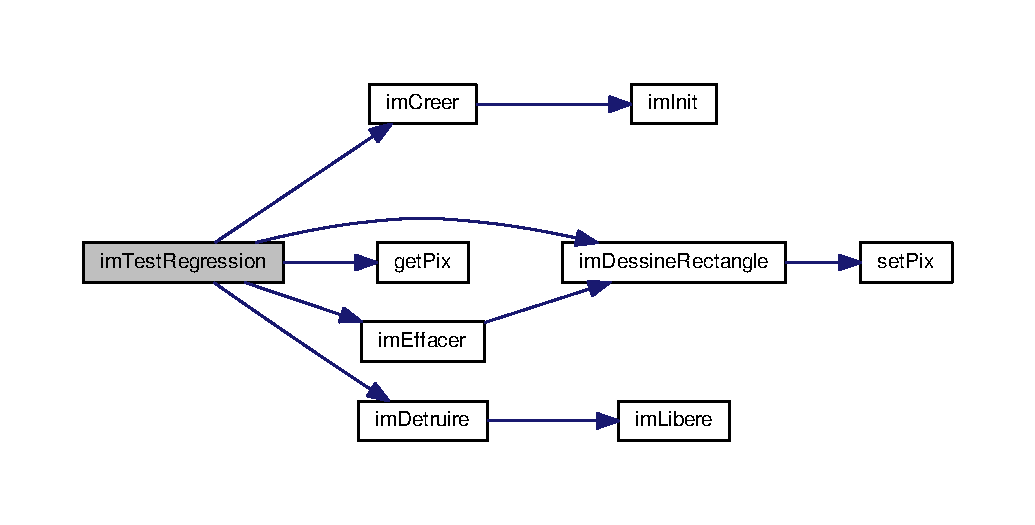
\includegraphics[width=350pt]{Image_8c_a8d4964490fb1a67b590ce77acd78031f_cgraph}
\end{center}
\end{figure}




Here is the caller graph for this function\+:\nopagebreak
\begin{figure}[H]
\begin{center}
\leavevmode
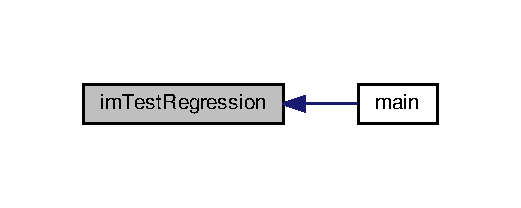
\includegraphics[width=250pt]{Image_8c_a8d4964490fb1a67b590ce77acd78031f_icgraph}
\end{center}
\end{figure}


\hypertarget{Image_8c_a7da553849b645f075994622df5bca888}{}\index{Image.\+c@{Image.\+c}!set\+Pix@{set\+Pix}}
\index{set\+Pix@{set\+Pix}!Image.\+c@{Image.\+c}}
\subsubsection[{set\+Pix}]{\setlength{\rightskip}{0pt plus 5cm}void set\+Pix (
\begin{DoxyParamCaption}
\item[{{\bf Image} $\ast$}]{im, }
\item[{const int}]{x, }
\item[{const int}]{y, }
\item[{{\bf Pixel}}]{couleur}
\end{DoxyParamCaption}
)}\label{Image_8c_a7da553849b645f075994622df5bca888}


set\+Pix modifie le pixel de coordonnées (x,y) 


\begin{DoxyParams}[1]{Parameters}
\mbox{\tt in,out}  & {\em im} & la structure image \\
\hline
\mbox{\tt in}  & {\em x} & Entier qui désigne les cordonnée de l\textquotesingle{}image sur l\textquotesingle{}axe des x \\
\hline
\mbox{\tt in}  & {\em y} & Entier qui désigne les cordonnée de l\textquotesingle{}image sur l\textquotesingle{}axe des y \\
\hline
\end{DoxyParams}
\begin{DoxyReturn}{Returns}
none.
\end{DoxyReturn}

\begin{DoxyCode}
1 setPix(&im,200,352);
\end{DoxyCode}
 \begin{DoxyWarning}{Warning}
x et y doivent etre inclu dans l\textquotesingle{}intervalle des dimensions 
\end{DoxyWarning}


Definition at line 63 of file Image.\+c.


\begin{DoxyCode}
64 \{
65     assert((x<im->dimx) && (y<im->dimy) && (x>=0) & (y>=0));
66 
67     im->\hyperlink{structImage_aad00390430c4e4e3a5a71bb919a4076c}{tab}[x][y]=couleur;
68 
69 
70 \}
\end{DoxyCode}


Here is the caller graph for this function\+:\nopagebreak
\begin{figure}[H]
\begin{center}
\leavevmode
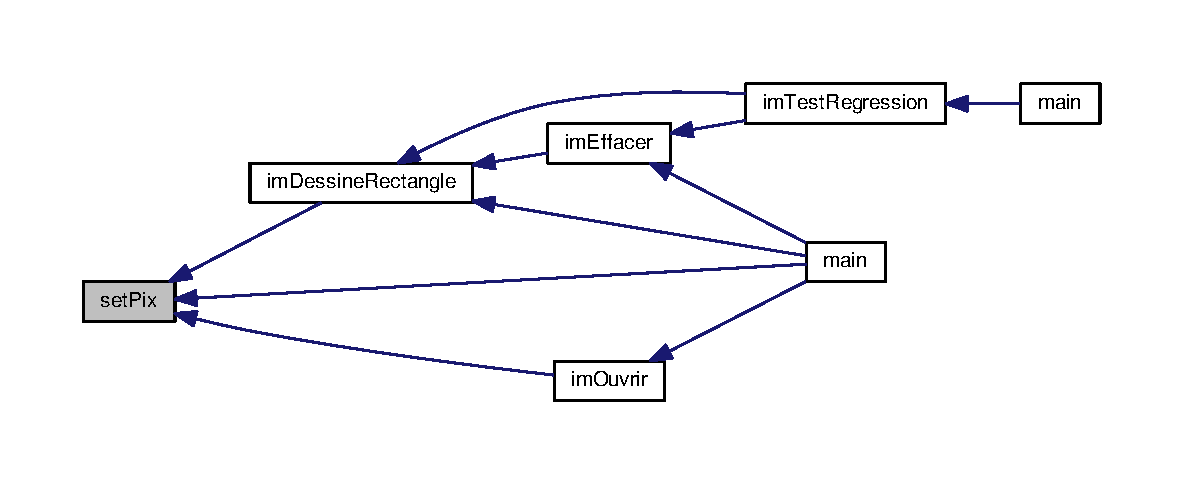
\includegraphics[width=350pt]{Image_8c_a7da553849b645f075994622df5bca888_icgraph}
\end{center}
\end{figure}



\hypertarget{Image_8h}{}\section{/home/wadi2a/\+Desktop/11512099/src/\+Image.h File Reference}
\label{Image_8h}\index{/home/wadi2a/\+Desktop/11512099/src/\+Image.\+h@{/home/wadi2a/\+Desktop/11512099/src/\+Image.\+h}}


Fichier .h du Module \hyperlink{structImage}{Image} Fichier qui comporte tout la déclaration des fonctions de ce module.  


{\ttfamily \#include \char`\"{}Pixel.\+h\char`\"{}}\\*
Include dependency graph for Image.\+h\+:\nopagebreak
\begin{figure}[H]
\begin{center}
\leavevmode
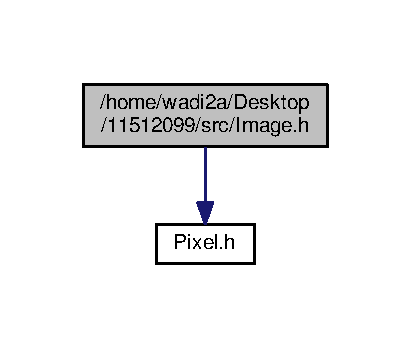
\includegraphics[width=197pt]{Image_8h__incl}
\end{center}
\end{figure}
This graph shows which files directly or indirectly include this file\+:\nopagebreak
\begin{figure}[H]
\begin{center}
\leavevmode
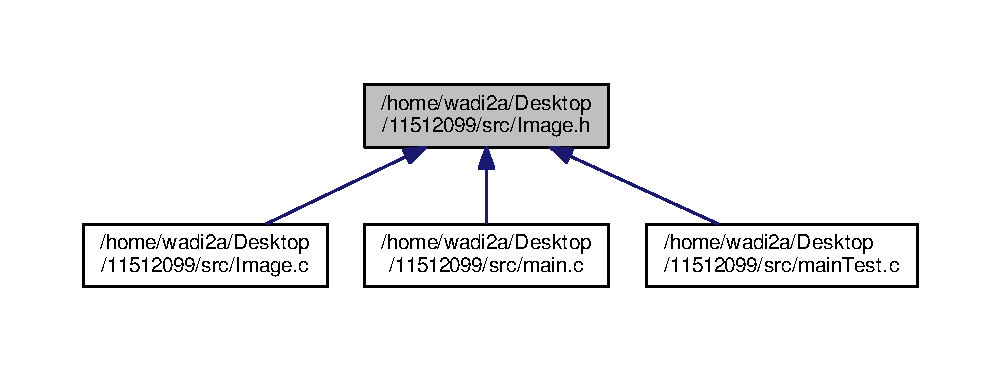
\includegraphics[width=350pt]{Image_8h__dep__incl}
\end{center}
\end{figure}
\subsection*{Data Structures}
\begin{DoxyCompactItemize}
\item 
struct \hyperlink{structImage}{Image}
\end{DoxyCompactItemize}
\subsection*{Typedefs}
\begin{DoxyCompactItemize}
\item 
typedef struct \hyperlink{structImage}{Image} \hyperlink{Image_8h_acf12205a65321baefe5174db248f56f6}{Image}
\end{DoxyCompactItemize}
\subsection*{Functions}
\begin{DoxyCompactItemize}
\item 
void \hyperlink{Image_8h_a6edbdf3bfe3beb4e44246a6c7985055c}{im\+Init} (\hyperlink{structImage}{Image} $\ast$im, const int dimx, const int dimy)
\begin{DoxyCompactList}\small\item\em im\+Init initialise dimx et dimy (après vérification) de la structure \hyperlink{structImage}{Image} puis alloue le tableau de pixel dans le tas \end{DoxyCompactList}\item 
void \hyperlink{Image_8h_a5931290abc22d365ae351381c594613f}{im\+Libere} (\hyperlink{structImage}{Image} $\ast$im)
\begin{DoxyCompactList}\small\item\em im\+Libere Libère la mémoire du tableau de pixels et met les champs dimx et dimy de la structure à 0 \end{DoxyCompactList}\item 
\hyperlink{structImage}{Image} $\ast$ \hyperlink{Image_8h_acd1b5e5f7a7fa80087a1e53bfa4da49d}{im\+Creer} (const int dimx, const int dimy)
\begin{DoxyCompactList}\small\item\em im\+Creer alloue dans le tas une structure \hyperlink{structImage}{Image} puis l\textquotesingle{}initialise avec im\+Init avant de la retourner \end{DoxyCompactList}\item 
void \hyperlink{Image_8h_acf3867531d803daad076cf18d2a14935}{im\+Detruire} (\hyperlink{structImage}{Image} $\ast$pim)
\begin{DoxyCompactList}\small\item\em im\+Detruire Libere le tableau de pixel en appelant im\+Libere puis détruit la structure image \end{DoxyCompactList}\item 
\hyperlink{structPixel}{Pixel} \hyperlink{Image_8h_a1cb04a46ed83be9a0c49b3b884c91d62}{get\+Pix} (const \hyperlink{structImage}{Image} $\ast$im, const int x, const int y)
\begin{DoxyCompactList}\small\item\em get\+Pix récupère le pixel de coordonnées (x,y) en vérifiant leur validité \end{DoxyCompactList}\item 
void \hyperlink{Image_8h_a7da553849b645f075994622df5bca888}{set\+Pix} (\hyperlink{structImage}{Image} $\ast$im, const int x, const int y, \hyperlink{structPixel}{Pixel} couleur)
\begin{DoxyCompactList}\small\item\em set\+Pix modifie le pixel de coordonnées (x,y) \end{DoxyCompactList}\item 
void \hyperlink{Image_8h_a44937c2130f18bd4a14481a5446d6e80}{im\+Dessine\+Rectangle} (\hyperlink{structImage}{Image} $\ast$im, const int Xmin, const int Ymin, const int Xmax, const int Ymax, const \hyperlink{structPixel}{Pixel} couleur)
\begin{DoxyCompactList}\small\item\em im\+Dessine\+Rectangle dessine un rectangle de couleur dans l\textquotesingle{}image en utilisant set\+Pix \end{DoxyCompactList}\item 
void \hyperlink{Image_8h_ae11c1ca640aae91cb1419158ad5bdf59}{im\+Effacer} (\hyperlink{structImage}{Image} $\ast$im, const \hyperlink{structPixel}{Pixel} couleur)
\begin{DoxyCompactList}\small\item\em im\+Effacer efface l\textquotesingle{}image en appelant im\+Dessine\+Rectangle avec le bon rectangle \end{DoxyCompactList}\item 
void \hyperlink{Image_8h_a20b9ad35b6db7bd09d7452574d04dd50}{im\+Sauver} (const \hyperlink{structImage}{Image} $\ast$p\+Im, const char filename\mbox{[}$\,$\mbox{]})
\begin{DoxyCompactList}\small\item\em im\+Sauver Enregistre l\textquotesingle{}image \end{DoxyCompactList}\item 
void \hyperlink{Image_8h_a0a1f0b9be4b910e1cfc2648cfa9e38fd}{im\+Ouvrir} (\hyperlink{structImage}{Image} $\ast$p\+Im, const char filename\mbox{[}$\,$\mbox{]})
\begin{DoxyCompactList}\small\item\em im\+Ouvrir ouvre l\textquotesingle{}image \end{DoxyCompactList}\item 
void \hyperlink{Image_8h_afadf8ab43119d304c72e201d0d95164d}{im\+Printf} (const \hyperlink{structImage}{Image} $\ast$p\+Im)
\begin{DoxyCompactList}\small\item\em im\+Printf affiche le contenue de chaque pixel dans l\textquotesingle{}image \end{DoxyCompactList}\item 
void \hyperlink{Image_8h_a8d4964490fb1a67b590ce77acd78031f}{im\+Test\+Regression} ()
\begin{DoxyCompactList}\small\item\em im\+Test\+Regression Effectue une série de tests vérifiant que le module fonctionne et que les champs de la structure sont conformes \end{DoxyCompactList}\end{DoxyCompactItemize}


\subsection{Detailed Description}
Fichier .h du Module \hyperlink{structImage}{Image} Fichier qui comporte tout la déclaration des fonctions de ce module. 

\begin{DoxyAuthor}{Author}
B\+E\+N A\+I\+S\+S\+A O\+U\+A\+D\+I\+E
\end{DoxyAuthor}
\begin{DoxyVersion}{Version}
1.\+0 
\end{DoxyVersion}
\begin{DoxyDate}{Date}
2016/02/10 
\end{DoxyDate}


\subsection{Typedef Documentation}
\hypertarget{Image_8h_acf12205a65321baefe5174db248f56f6}{}\index{Image.\+h@{Image.\+h}!Image@{Image}}
\index{Image@{Image}!Image.\+h@{Image.\+h}}
\subsubsection[{Image}]{\setlength{\rightskip}{0pt plus 5cm}typedef struct {\bf Image} {\bf Image}}\label{Image_8h_acf12205a65321baefe5174db248f56f6}


Definition at line 20 of file Image.\+h.



\subsection{Function Documentation}
\hypertarget{Image_8h_a1cb04a46ed83be9a0c49b3b884c91d62}{}\index{Image.\+h@{Image.\+h}!get\+Pix@{get\+Pix}}
\index{get\+Pix@{get\+Pix}!Image.\+h@{Image.\+h}}
\subsubsection[{get\+Pix}]{\setlength{\rightskip}{0pt plus 5cm}{\bf Pixel} get\+Pix (
\begin{DoxyParamCaption}
\item[{const {\bf Image} $\ast$}]{im, }
\item[{const int}]{x, }
\item[{const int}]{y}
\end{DoxyParamCaption}
)}\label{Image_8h_a1cb04a46ed83be9a0c49b3b884c91d62}


get\+Pix récupère le pixel de coordonnées (x,y) en vérifiant leur validité 


\begin{DoxyParams}[1]{Parameters}
\mbox{\tt in,out}  & {\em im} & la structure image \\
\hline
\mbox{\tt in}  & {\em x} & Entier qui désigne les cordonnée de l\textquotesingle{}image sur l\textquotesingle{}axe des x \\
\hline
\mbox{\tt in}  & {\em y} & Entier qui désigne les cordonnée de l\textquotesingle{}image sur l\textquotesingle{}axe des y \\
\hline
\end{DoxyParams}
\begin{DoxyReturn}{Returns}
lien vers une pixel.
\end{DoxyReturn}

\begin{DoxyCode}
1 getPix(&im,200,352);
\end{DoxyCode}
 \begin{DoxyWarning}{Warning}
x et y doivent etre inclu dans l\textquotesingle{}intervalle des dimensions 
\end{DoxyWarning}


Definition at line 55 of file Image.\+c.


\begin{DoxyCode}
56 \{
57 
58     assert(x<im->dimx && y<im->dimy);
59     \textcolor{keywordflow}{return} im->\hyperlink{structImage_aad00390430c4e4e3a5a71bb919a4076c}{tab}[x][y];
60 
61 \}
\end{DoxyCode}


Here is the caller graph for this function\+:\nopagebreak
\begin{figure}[H]
\begin{center}
\leavevmode
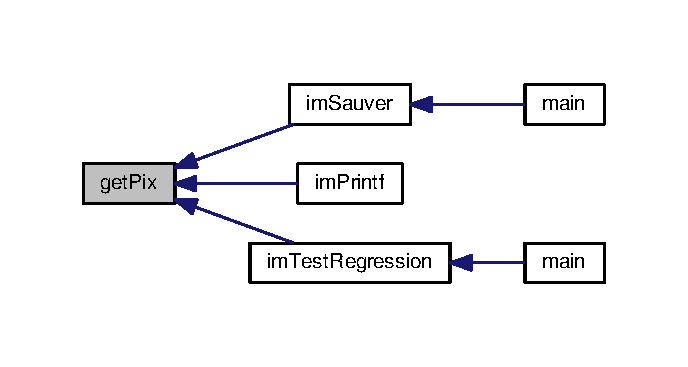
\includegraphics[width=330pt]{Image_8h_a1cb04a46ed83be9a0c49b3b884c91d62_icgraph}
\end{center}
\end{figure}


\hypertarget{Image_8h_acd1b5e5f7a7fa80087a1e53bfa4da49d}{}\index{Image.\+h@{Image.\+h}!im\+Creer@{im\+Creer}}
\index{im\+Creer@{im\+Creer}!Image.\+h@{Image.\+h}}
\subsubsection[{im\+Creer}]{\setlength{\rightskip}{0pt plus 5cm}{\bf Image}$\ast$ im\+Creer (
\begin{DoxyParamCaption}
\item[{const int}]{dimx, }
\item[{const int}]{dimy}
\end{DoxyParamCaption}
)}\label{Image_8h_acd1b5e5f7a7fa80087a1e53bfa4da49d}


im\+Creer alloue dans le tas une structure \hyperlink{structImage}{Image} puis l\textquotesingle{}initialise avec im\+Init avant de la retourner 


\begin{DoxyParams}[1]{Parameters}
\mbox{\tt in}  & {\em dimx} & Entier qui désigne la largeur de l\textquotesingle{}image. \\
\hline
\mbox{\tt in}  & {\em dimy} & Entier qui désigne la hauteur de l\textquotesingle{}image. \\
\hline
\end{DoxyParams}
\begin{DoxyReturn}{Returns}
lien sur image. 
\begin{DoxyCode}
1 imCreer(500,500);
\end{DoxyCode}
 
\end{DoxyReturn}
\begin{DoxyWarning}{Warning}
les dimension de l\textquotesingle{}image doivent etre dimx$>$0 et dimy$>$0 
\end{DoxyWarning}


Definition at line 40 of file Image.\+c.


\begin{DoxyCode}
41 \{
42     \hyperlink{structImage}{Image} * im=malloc( \textcolor{keyword}{sizeof}(\hyperlink{structImage}{Image}));
43 
44     \hyperlink{Image_8c_a6edbdf3bfe3beb4e44246a6c7985055c}{imInit}(im,dimx,dimy);
45     \textcolor{keywordflow}{return} im;
46 \}
\end{DoxyCode}


Here is the call graph for this function\+:\nopagebreak
\begin{figure}[H]
\begin{center}
\leavevmode
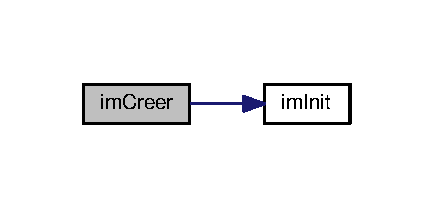
\includegraphics[width=208pt]{Image_8h_acd1b5e5f7a7fa80087a1e53bfa4da49d_cgraph}
\end{center}
\end{figure}




Here is the caller graph for this function\+:\nopagebreak
\begin{figure}[H]
\begin{center}
\leavevmode
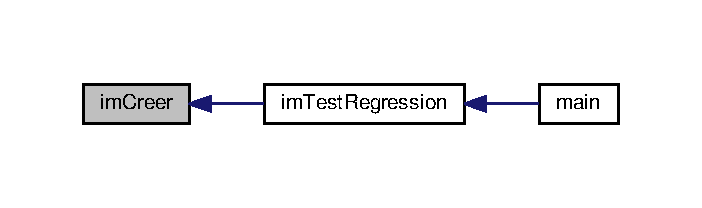
\includegraphics[width=337pt]{Image_8h_acd1b5e5f7a7fa80087a1e53bfa4da49d_icgraph}
\end{center}
\end{figure}


\hypertarget{Image_8h_a44937c2130f18bd4a14481a5446d6e80}{}\index{Image.\+h@{Image.\+h}!im\+Dessine\+Rectangle@{im\+Dessine\+Rectangle}}
\index{im\+Dessine\+Rectangle@{im\+Dessine\+Rectangle}!Image.\+h@{Image.\+h}}
\subsubsection[{im\+Dessine\+Rectangle}]{\setlength{\rightskip}{0pt plus 5cm}void im\+Dessine\+Rectangle (
\begin{DoxyParamCaption}
\item[{{\bf Image} $\ast$}]{im, }
\item[{const int}]{Xmin, }
\item[{const int}]{Ymin, }
\item[{const int}]{Xmax, }
\item[{const int}]{Ymax, }
\item[{const {\bf Pixel}}]{couleur}
\end{DoxyParamCaption}
)}\label{Image_8h_a44937c2130f18bd4a14481a5446d6e80}


im\+Dessine\+Rectangle dessine un rectangle de couleur dans l\textquotesingle{}image en utilisant set\+Pix 


\begin{DoxyParams}[1]{Parameters}
\mbox{\tt in,out}  & {\em im} & la structure image \\
\hline
\mbox{\tt in}  & {\em Xmin} & Entier qui désigne le début du rectangle sur l\textquotesingle{}axe des x \\
\hline
\mbox{\tt in}  & {\em Xmax} & Entier qui désigne la fin du rectangle sur l\textquotesingle{}axe des x \\
\hline
\mbox{\tt in}  & {\em Ymin} & Entier qui désigne le début du rectangle sur l\textquotesingle{}axe des y \\
\hline
\mbox{\tt in}  & {\em Ymax} & Entier qui désigne la fin du rectangle sur l\textquotesingle{}axe des x \\
\hline
\mbox{\tt in}  & {\em couleur} & \hyperlink{structPixel}{Pixel} qui contient les valeurs du couleurs que nous allons l\textquotesingle{}affecté au triangle \\
\hline
\end{DoxyParams}
\begin{DoxyReturn}{Returns}
none.
\end{DoxyReturn}

\begin{DoxyCode}
1 imDessineRectangle(&im,100,100,200,352,couleur);
\end{DoxyCode}
 \begin{DoxyWarning}{Warning}
Xmin,Xmax,Ymin,Ymax doivent etre inclu dans l\textquotesingle{}intervalle des dimensions 
\end{DoxyWarning}


Definition at line 72 of file Image.\+c.


\begin{DoxyCode}
73 \{   \textcolor{keywordtype}{int} i=0,j=0;
74     assert((Xmin>=0) && (Xmax<im->dimx) && (Ymin>=0) && (Ymax<im->dimy));
75     \textcolor{comment}{/*}
76 \textcolor{comment}{    pour dessiner un triangle vide a l'interieur}
77 \textcolor{comment}{    for(i=Xmin;i<=Xmax;i++) setPix(im,i,Ymin,couleur);}
78 \textcolor{comment}{    for(i=Ymin;i<=Ymax;i++) setPix(im,Xmin,i,couleur);}
79 \textcolor{comment}{    for(i=Xmin;i<=Xmax;i++) setPix(im,i,Ymax,couleur);}
80 \textcolor{comment}{    for(i=Ymin;i<=Ymax;i++) setPix(im,Xmax,i,couleur);*/}
81     \textcolor{keywordflow}{for}(i=Xmin;i<=Xmax;i++)
82     \{
83         \textcolor{keywordflow}{for}(j=Ymin;j<=Ymax;j++)
84         \{
85             \hyperlink{Image_8c_a7da553849b645f075994622df5bca888}{setPix}(im,i,j,couleur);
86         \}
87     \}
88 \}
\end{DoxyCode}


Here is the call graph for this function\+:\nopagebreak
\begin{figure}[H]
\begin{center}
\leavevmode
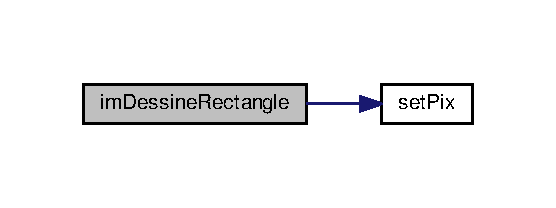
\includegraphics[width=267pt]{Image_8h_a44937c2130f18bd4a14481a5446d6e80_cgraph}
\end{center}
\end{figure}




Here is the caller graph for this function\+:\nopagebreak
\begin{figure}[H]
\begin{center}
\leavevmode
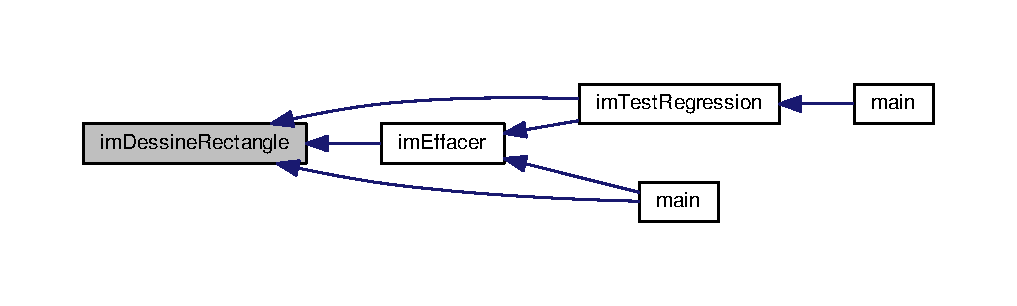
\includegraphics[width=350pt]{Image_8h_a44937c2130f18bd4a14481a5446d6e80_icgraph}
\end{center}
\end{figure}


\hypertarget{Image_8h_acf3867531d803daad076cf18d2a14935}{}\index{Image.\+h@{Image.\+h}!im\+Detruire@{im\+Detruire}}
\index{im\+Detruire@{im\+Detruire}!Image.\+h@{Image.\+h}}
\subsubsection[{im\+Detruire}]{\setlength{\rightskip}{0pt plus 5cm}void im\+Detruire (
\begin{DoxyParamCaption}
\item[{{\bf Image} $\ast$}]{pim}
\end{DoxyParamCaption}
)}\label{Image_8h_acf3867531d803daad076cf18d2a14935}


im\+Detruire Libere le tableau de pixel en appelant im\+Libere puis détruit la structure image 


\begin{DoxyParams}[1]{Parameters}
\mbox{\tt in,out}  & {\em im} & la structure image à détruire. \\
\hline
\end{DoxyParams}
\begin{DoxyReturn}{Returns}
none. 
\begin{DoxyCode}
1 imDetruire(Image *pim);
\end{DoxyCode}
 
\end{DoxyReturn}


Definition at line 48 of file Image.\+c.


\begin{DoxyCode}
49 \{
50     \hyperlink{Image_8c_a5931290abc22d365ae351381c594613f}{imLibere}(pim);
51     free(pim);
52 
53 
54 \}
\end{DoxyCode}


Here is the call graph for this function\+:\nopagebreak
\begin{figure}[H]
\begin{center}
\leavevmode
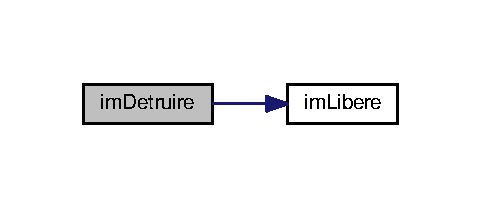
\includegraphics[width=231pt]{Image_8h_acf3867531d803daad076cf18d2a14935_cgraph}
\end{center}
\end{figure}




Here is the caller graph for this function\+:\nopagebreak
\begin{figure}[H]
\begin{center}
\leavevmode
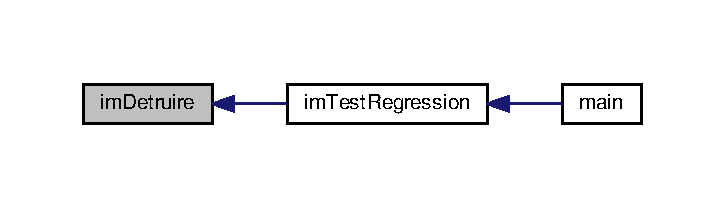
\includegraphics[width=348pt]{Image_8h_acf3867531d803daad076cf18d2a14935_icgraph}
\end{center}
\end{figure}


\hypertarget{Image_8h_ae11c1ca640aae91cb1419158ad5bdf59}{}\index{Image.\+h@{Image.\+h}!im\+Effacer@{im\+Effacer}}
\index{im\+Effacer@{im\+Effacer}!Image.\+h@{Image.\+h}}
\subsubsection[{im\+Effacer}]{\setlength{\rightskip}{0pt plus 5cm}void im\+Effacer (
\begin{DoxyParamCaption}
\item[{{\bf Image} $\ast$}]{im, }
\item[{const {\bf Pixel}}]{couleur}
\end{DoxyParamCaption}
)}\label{Image_8h_ae11c1ca640aae91cb1419158ad5bdf59}


im\+Effacer efface l\textquotesingle{}image en appelant im\+Dessine\+Rectangle avec le bon rectangle 


\begin{DoxyParams}[1]{Parameters}
\mbox{\tt in,out}  & {\em im} & la structure image \\
\hline
\mbox{\tt in}  & {\em couleur} & \hyperlink{structPixel}{Pixel} qui contient les valeurs du couleurs que nous allons l\textquotesingle{}affecté au triangle \\
\hline
\end{DoxyParams}
\begin{DoxyReturn}{Returns}
none.
\end{DoxyReturn}

\begin{DoxyCode}
1 imEffacer(&im,couleur);
\end{DoxyCode}
 

Definition at line 89 of file Image.\+c.


\begin{DoxyCode}
90 \{
91 
92     \hyperlink{Image_8c_a01084dc5c10d366999aece5432dc823f}{imDessineRectangle}(im,0,0,im->\hyperlink{structImage_a1fbf685f50372de48b7290cd02a77b0c}{dimx}-1,im->\hyperlink{structImage_a2e937e4780121e32bce2ccae87069b68}{dimy}-1,couleur);
93 
94 \}
\end{DoxyCode}


Here is the call graph for this function\+:\nopagebreak
\begin{figure}[H]
\begin{center}
\leavevmode
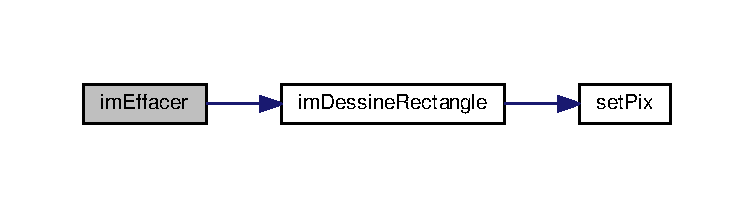
\includegraphics[width=350pt]{Image_8h_ae11c1ca640aae91cb1419158ad5bdf59_cgraph}
\end{center}
\end{figure}




Here is the caller graph for this function\+:\nopagebreak
\begin{figure}[H]
\begin{center}
\leavevmode
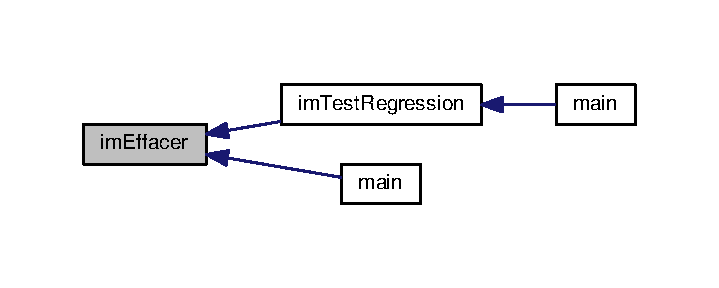
\includegraphics[width=345pt]{Image_8h_ae11c1ca640aae91cb1419158ad5bdf59_icgraph}
\end{center}
\end{figure}


\hypertarget{Image_8h_a6edbdf3bfe3beb4e44246a6c7985055c}{}\index{Image.\+h@{Image.\+h}!im\+Init@{im\+Init}}
\index{im\+Init@{im\+Init}!Image.\+h@{Image.\+h}}
\subsubsection[{im\+Init}]{\setlength{\rightskip}{0pt plus 5cm}void im\+Init (
\begin{DoxyParamCaption}
\item[{{\bf Image} $\ast$}]{im, }
\item[{const int}]{dimx, }
\item[{const int}]{dimy}
\end{DoxyParamCaption}
)}\label{Image_8h_a6edbdf3bfe3beb4e44246a6c7985055c}


im\+Init initialise dimx et dimy (après vérification) de la structure \hyperlink{structImage}{Image} puis alloue le tableau de pixel dans le tas 


\begin{DoxyParams}[1]{Parameters}
\mbox{\tt in,out}  & {\em im} & la structure image à initialisé \\
\hline
\mbox{\tt in}  & {\em dimx} & Entier qui désigne la largeur de l\textquotesingle{}image \\
\hline
\mbox{\tt in}  & {\em dimy} & Entier qui désigne la hauteur de l\textquotesingle{}image \\
\hline
\end{DoxyParams}
\begin{DoxyReturn}{Returns}
none.
\end{DoxyReturn}

\begin{DoxyCode}
1 imInit(&im,500,500);
\end{DoxyCode}
 \begin{DoxyWarning}{Warning}
les dimension de l\textquotesingle{}image doivent etre dimx$>$0 et dimy$>$0 
\end{DoxyWarning}


Definition at line 15 of file Image.\+c.


\begin{DoxyCode}
16 \{
17     \textcolor{keywordtype}{int} i;
18 
19     assert(dimx>0 && dimy>0);
20     im->\hyperlink{structImage_aad00390430c4e4e3a5a71bb919a4076c}{tab}=malloc(dimy * \textcolor{keyword}{sizeof}(\hyperlink{structPixel}{Pixel}*));
21     \textcolor{keywordflow}{for}(i=0;i<dimy;i++)
22     \{
23         im->\hyperlink{structImage_aad00390430c4e4e3a5a71bb919a4076c}{tab}[i]=(\hyperlink{structPixel}{Pixel}*)malloc(dimy*\textcolor{keyword}{sizeof}(\hyperlink{structPixel}{Pixel}));
24     \}
25     im->\hyperlink{structImage_a1fbf685f50372de48b7290cd02a77b0c}{dimx}=dimx;
26     im->\hyperlink{structImage_a2e937e4780121e32bce2ccae87069b68}{dimy}=dimy;
27  
28 \}
\end{DoxyCode}


Here is the caller graph for this function\+:\nopagebreak
\begin{figure}[H]
\begin{center}
\leavevmode
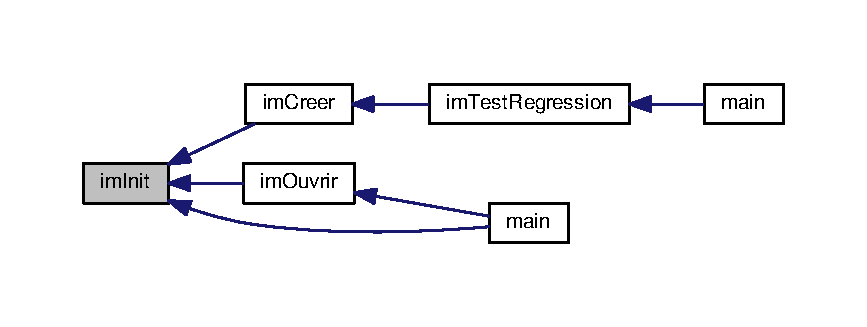
\includegraphics[width=350pt]{Image_8h_a6edbdf3bfe3beb4e44246a6c7985055c_icgraph}
\end{center}
\end{figure}


\hypertarget{Image_8h_a5931290abc22d365ae351381c594613f}{}\index{Image.\+h@{Image.\+h}!im\+Libere@{im\+Libere}}
\index{im\+Libere@{im\+Libere}!Image.\+h@{Image.\+h}}
\subsubsection[{im\+Libere}]{\setlength{\rightskip}{0pt plus 5cm}void im\+Libere (
\begin{DoxyParamCaption}
\item[{{\bf Image} $\ast$}]{im}
\end{DoxyParamCaption}
)}\label{Image_8h_a5931290abc22d365ae351381c594613f}


im\+Libere Libère la mémoire du tableau de pixels et met les champs dimx et dimy de la structure à 0 


\begin{DoxyParams}[1]{Parameters}
\mbox{\tt in,out}  & {\em im} & la structure image à initialisé. \\
\hline
\end{DoxyParams}
\begin{DoxyReturn}{Returns}
none. 
\begin{DoxyCode}
1 void imLibere(&im);
\end{DoxyCode}
 
\end{DoxyReturn}


Definition at line 30 of file Image.\+c.


\begin{DoxyCode}
31 \{   \textcolor{keywordtype}{int} i;
32     \textcolor{keywordflow}{for}(i=0;i<im->\hyperlink{structImage_a2e937e4780121e32bce2ccae87069b68}{dimy};i++)
33     \{
34         free(im->\hyperlink{structImage_aad00390430c4e4e3a5a71bb919a4076c}{tab}[i]);
35     \}
36 
37     im->\hyperlink{structImage_a1fbf685f50372de48b7290cd02a77b0c}{dimx}=0;
38     im->\hyperlink{structImage_a2e937e4780121e32bce2ccae87069b68}{dimy}=0;
39 \}
\end{DoxyCode}


Here is the caller graph for this function\+:\nopagebreak
\begin{figure}[H]
\begin{center}
\leavevmode
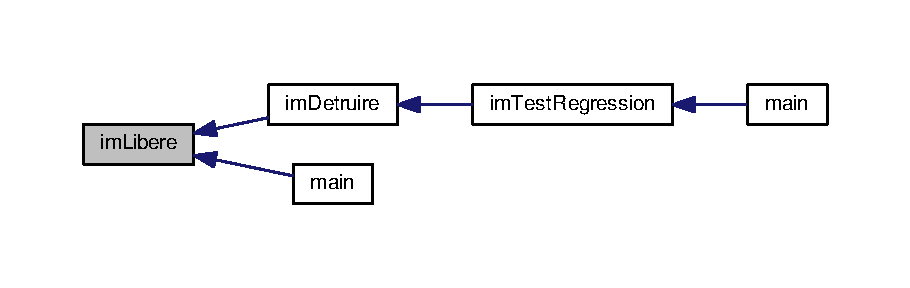
\includegraphics[width=350pt]{Image_8h_a5931290abc22d365ae351381c594613f_icgraph}
\end{center}
\end{figure}


\hypertarget{Image_8h_a0a1f0b9be4b910e1cfc2648cfa9e38fd}{}\index{Image.\+h@{Image.\+h}!im\+Ouvrir@{im\+Ouvrir}}
\index{im\+Ouvrir@{im\+Ouvrir}!Image.\+h@{Image.\+h}}
\subsubsection[{im\+Ouvrir}]{\setlength{\rightskip}{0pt plus 5cm}void im\+Ouvrir (
\begin{DoxyParamCaption}
\item[{{\bf Image} $\ast$}]{p\+Im, }
\item[{const char}]{filename\mbox{[}$\,$\mbox{]}}
\end{DoxyParamCaption}
)}\label{Image_8h_a0a1f0b9be4b910e1cfc2648cfa9e38fd}


im\+Ouvrir ouvre l\textquotesingle{}image 


\begin{DoxyParams}[1]{Parameters}
\mbox{\tt in,out}  & {\em im} & la structure image \\
\hline
\mbox{\tt in}  & {\em chaine} & de caractère qui désigne l\textquotesingle{}emplacement de l\textquotesingle{}image \\
\hline
\end{DoxyParams}
\begin{DoxyReturn}{Returns}
none.
\end{DoxyReturn}

\begin{DoxyCode}
1 imOuvrir(&im,"./data/toto.ppm");
\end{DoxyCode}
 \begin{DoxyWarning}{Warning}
l\textquotesingle{}image doit etre crée avant l\textquotesingle{}execution de cette procedure 
\end{DoxyWarning}


Definition at line 118 of file Image.\+c.


\begin{DoxyCode}
118                                                  \{
119     FILE* f;
120     \hyperlink{structPixel}{Pixel} pix;
121     \textcolor{keywordtype}{int} x, y, dimx, dimy;
122 
123     f = fopen(filename, \textcolor{stringliteral}{"r"});
124     \textcolor{keywordflow}{if} (f==NULL) \{
125         printf(\textcolor{stringliteral}{"Erreur lors de l'ouverture de %s\(\backslash\)n"}, filename);
126         assert( f );
127     \}
128 
129     assert( fscanf( f , \textcolor{stringliteral}{"P3\(\backslash\)n%d %d\(\backslash\)n255\(\backslash\)n"}, &dimx, &dimy) == 2 );
130     \hyperlink{Image_8c_a6edbdf3bfe3beb4e44246a6c7985055c}{imInit}( pIm, dimx, dimy);
131 
132     \textcolor{keywordflow}{for}(y=0;y<pIm->\hyperlink{structImage_a2e937e4780121e32bce2ccae87069b68}{dimy};++y)
133         \textcolor{keywordflow}{for}(x=0;x<pIm->\hyperlink{structImage_a1fbf685f50372de48b7290cd02a77b0c}{dimx};++x) \{
134             assert( fscanf(f, \textcolor{stringliteral}{"%c %c %c  "}, &pix.\hyperlink{structPixel_a038ad5b3349e7548d17c5d3bec511b94}{r}, &pix.\hyperlink{structPixel_a8407845aacf1663d9463475619911686}{g}, &pix.\hyperlink{structPixel_a760bdf29b15433d257f119239fcff4d4}{b}) == 3 );
135             \hyperlink{Image_8c_a7da553849b645f075994622df5bca888}{setPix}(pIm,x,y,pix);
136         \}
137     fclose(f);
138     printf(\textcolor{stringliteral}{"Lecture de l'image %s ...OK\(\backslash\)n"}, filename);
139 \}
\end{DoxyCode}


Here is the call graph for this function\+:\nopagebreak
\begin{figure}[H]
\begin{center}
\leavevmode
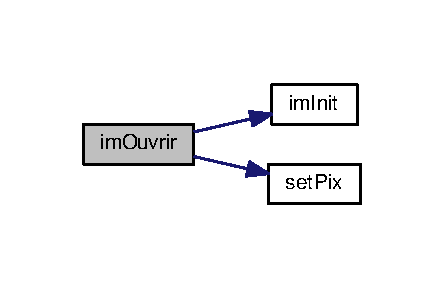
\includegraphics[width=213pt]{Image_8h_a0a1f0b9be4b910e1cfc2648cfa9e38fd_cgraph}
\end{center}
\end{figure}




Here is the caller graph for this function\+:\nopagebreak
\begin{figure}[H]
\begin{center}
\leavevmode
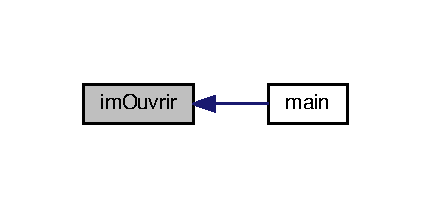
\includegraphics[width=207pt]{Image_8h_a0a1f0b9be4b910e1cfc2648cfa9e38fd_icgraph}
\end{center}
\end{figure}


\hypertarget{Image_8h_afadf8ab43119d304c72e201d0d95164d}{}\index{Image.\+h@{Image.\+h}!im\+Printf@{im\+Printf}}
\index{im\+Printf@{im\+Printf}!Image.\+h@{Image.\+h}}
\subsubsection[{im\+Printf}]{\setlength{\rightskip}{0pt plus 5cm}void im\+Printf (
\begin{DoxyParamCaption}
\item[{const {\bf Image} $\ast$}]{p\+Im}
\end{DoxyParamCaption}
)}\label{Image_8h_afadf8ab43119d304c72e201d0d95164d}


im\+Printf affiche le contenue de chaque pixel dans l\textquotesingle{}image 


\begin{DoxyParams}[1]{Parameters}
\mbox{\tt in,out}  & {\em im} & la structure image \\
\hline
\end{DoxyParams}
\begin{DoxyReturn}{Returns}
none.
\end{DoxyReturn}

\begin{DoxyCode}
1 imPrintf(&im);
\end{DoxyCode}
 \begin{DoxyWarning}{Warning}
l\textquotesingle{}image doit etre crée avant l\textquotesingle{}execution de cette procedure 
\end{DoxyWarning}


Definition at line 141 of file Image.\+c.


\begin{DoxyCode}
141                                 \{
142     \textcolor{keywordtype}{int} x,y;
143     \hyperlink{structPixel}{Pixel} pix;
144 
145     printf( \textcolor{stringliteral}{"%d %d\(\backslash\)n"}, pIm->\hyperlink{structImage_a1fbf685f50372de48b7290cd02a77b0c}{dimx}, pIm->\hyperlink{structImage_a2e937e4780121e32bce2ccae87069b68}{dimy});      \textcolor{comment}{/* dimension de l'image*/}
146 
147     \textcolor{keywordflow}{for}(y=0;y<pIm->\hyperlink{structImage_a2e937e4780121e32bce2ccae87069b68}{dimy};++y) \{
148         \textcolor{keywordflow}{for}(x=0;x<pIm->\hyperlink{structImage_a1fbf685f50372de48b7290cd02a77b0c}{dimx};++x) \{
149             pix = \hyperlink{Image_8c_a1cb04a46ed83be9a0c49b3b884c91d62}{getPix}(pIm,x,y);
150             printf(\textcolor{stringliteral}{"%d %d %d  "}, pix.\hyperlink{structPixel_a038ad5b3349e7548d17c5d3bec511b94}{r}, pix.\hyperlink{structPixel_a8407845aacf1663d9463475619911686}{g}, pix.\hyperlink{structPixel_a760bdf29b15433d257f119239fcff4d4}{b});
151         \}
152         printf(\textcolor{stringliteral}{"\(\backslash\)n"});
153     \}
154 \}
\end{DoxyCode}


Here is the call graph for this function\+:\nopagebreak
\begin{figure}[H]
\begin{center}
\leavevmode
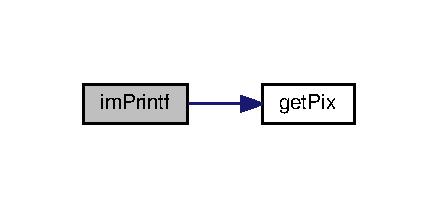
\includegraphics[width=210pt]{Image_8h_afadf8ab43119d304c72e201d0d95164d_cgraph}
\end{center}
\end{figure}


\hypertarget{Image_8h_a20b9ad35b6db7bd09d7452574d04dd50}{}\index{Image.\+h@{Image.\+h}!im\+Sauver@{im\+Sauver}}
\index{im\+Sauver@{im\+Sauver}!Image.\+h@{Image.\+h}}
\subsubsection[{im\+Sauver}]{\setlength{\rightskip}{0pt plus 5cm}void im\+Sauver (
\begin{DoxyParamCaption}
\item[{const {\bf Image} $\ast$}]{p\+Im, }
\item[{const char}]{filename\mbox{[}$\,$\mbox{]}}
\end{DoxyParamCaption}
)}\label{Image_8h_a20b9ad35b6db7bd09d7452574d04dd50}


im\+Sauver Enregistre l\textquotesingle{}image 


\begin{DoxyParams}[1]{Parameters}
\mbox{\tt in,out}  & {\em im} & la structure image \\
\hline
\mbox{\tt in}  & {\em chaine} & de caractère qui désigne l\textquotesingle{}emplacement de l\textquotesingle{}image \\
\hline
\end{DoxyParams}
\begin{DoxyReturn}{Returns}
none.
\end{DoxyReturn}

\begin{DoxyCode}
1 imSauver(&im,"./data/toto.ppm");
\end{DoxyCode}
 \begin{DoxyWarning}{Warning}
l\textquotesingle{}image doit etre crée avant l\textquotesingle{}execution de cette procedure 
\end{DoxyWarning}


Definition at line 96 of file Image.\+c.


\begin{DoxyCode}
96                                                        \{
97     FILE* f;
98     \hyperlink{structPixel}{Pixel} pix;
99     \textcolor{keywordtype}{int} x,y;
100 
101     f = fopen(filename, \textcolor{stringliteral}{"w"});
102     \textcolor{keywordflow}{if} (f==NULL) \{
103         printf(\textcolor{stringliteral}{"Erreur lors de l'ouverture de %s\(\backslash\)n"}, filename);
104         assert( f );
105     \}
106     fprintf( f , \textcolor{stringliteral}{"P3\(\backslash\)n"});                           \textcolor{comment}{/*P3 = ascii avec 3 composantes RGB*/}
107     fprintf( f , \textcolor{stringliteral}{"%d %d\(\backslash\)n"}, pIm->\hyperlink{structImage_a1fbf685f50372de48b7290cd02a77b0c}{dimx}, pIm->\hyperlink{structImage_a2e937e4780121e32bce2ccae87069b68}{dimy});  \textcolor{comment}{/* dimension de l'image*/}
108     fprintf( f , \textcolor{stringliteral}{"255\(\backslash\)n"});                          \textcolor{comment}{/* chaque composante est comprise entre 0 et 255*/}
109 
110     \textcolor{keywordflow}{for}(y=0;y<pIm->\hyperlink{structImage_a2e937e4780121e32bce2ccae87069b68}{dimy};++y)
111         \textcolor{keywordflow}{for}(x=0;x<pIm->\hyperlink{structImage_a1fbf685f50372de48b7290cd02a77b0c}{dimx};++x) \{
112             pix = \hyperlink{Image_8c_a1cb04a46ed83be9a0c49b3b884c91d62}{getPix}(pIm,x++,y);
113             fprintf(f, \textcolor{stringliteral}{"%d %d %d  "}, pix.\hyperlink{structPixel_a038ad5b3349e7548d17c5d3bec511b94}{r}, pix.\hyperlink{structPixel_a8407845aacf1663d9463475619911686}{g}, pix.\hyperlink{structPixel_a760bdf29b15433d257f119239fcff4d4}{b});
114         \}
115     printf(\textcolor{stringliteral}{"Sauvegarde de l'image %s ...OK\(\backslash\)n"}, filename);
116     fclose(f);
117 \}
\end{DoxyCode}


Here is the call graph for this function\+:\nopagebreak
\begin{figure}[H]
\begin{center}
\leavevmode
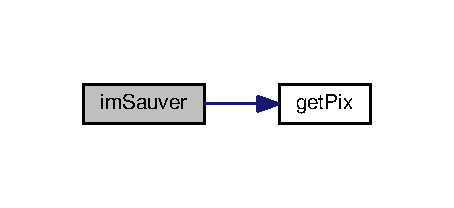
\includegraphics[width=218pt]{Image_8h_a20b9ad35b6db7bd09d7452574d04dd50_cgraph}
\end{center}
\end{figure}




Here is the caller graph for this function\+:\nopagebreak
\begin{figure}[H]
\begin{center}
\leavevmode
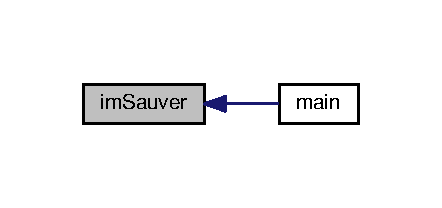
\includegraphics[width=212pt]{Image_8h_a20b9ad35b6db7bd09d7452574d04dd50_icgraph}
\end{center}
\end{figure}


\hypertarget{Image_8h_a8d4964490fb1a67b590ce77acd78031f}{}\index{Image.\+h@{Image.\+h}!im\+Test\+Regression@{im\+Test\+Regression}}
\index{im\+Test\+Regression@{im\+Test\+Regression}!Image.\+h@{Image.\+h}}
\subsubsection[{im\+Test\+Regression}]{\setlength{\rightskip}{0pt plus 5cm}void im\+Test\+Regression (
\begin{DoxyParamCaption}
{}
\end{DoxyParamCaption}
)}\label{Image_8h_a8d4964490fb1a67b590ce77acd78031f}


im\+Test\+Regression Effectue une série de tests vérifiant que le module fonctionne et que les champs de la structure sont conformes 


\begin{DoxyParams}{Parameters}
{\em none} & \\
\hline
\end{DoxyParams}
\begin{DoxyReturn}{Returns}
none.
\end{DoxyReturn}

\begin{DoxyCode}
1 imTestRegression();
\end{DoxyCode}
 

Definition at line 156 of file Image.\+c.


\begin{DoxyCode}
157 \{
158     \hyperlink{structImage}{Image} * im;
159     \textcolor{keywordtype}{int} dimx,dimy;\textcolor{keywordtype}{int} i,j;\hyperlink{structPixel}{Pixel} couleur2 = \{ 0, 0, 0 \};
160     \hyperlink{structPixel}{Pixel} couleur;couleur.\hyperlink{structPixel_a760bdf29b15433d257f119239fcff4d4}{b}=8;couleur.\hyperlink{structPixel_a038ad5b3349e7548d17c5d3bec511b94}{r}=1;couleur.\hyperlink{structPixel_a8407845aacf1663d9463475619911686}{g}=1;
161 
162     printf(\textcolor{stringliteral}{"Donnez la dimension de ton image:\(\backslash\)n dimx:"});
163     scanf(\textcolor{stringliteral}{"%d"},&dimx);
164     printf(\textcolor{stringliteral}{"dimy:"});
165     scanf(\textcolor{stringliteral}{"%d"},&dimy);
166     im=\hyperlink{Image_8c_acd1b5e5f7a7fa80087a1e53bfa4da49d}{imCreer}(dimx,dimy);
167     printf(\textcolor{stringliteral}{"Taille de l'image :%dpx*%dpx"},im->\hyperlink{structImage_a1fbf685f50372de48b7290cd02a77b0c}{dimx},im->\hyperlink{structImage_a2e937e4780121e32bce2ccae87069b68}{dimy});
168      \hyperlink{Image_8c_a01084dc5c10d366999aece5432dc823f}{imDessineRectangle}(im,4,6,12,15,couleur);printf(\textcolor{stringliteral}{"\(\backslash\)n"});
169      \textcolor{keywordflow}{for}(j=0;j<im->\hyperlink{structImage_a2e937e4780121e32bce2ccae87069b68}{dimy};j++)
170      \{
171         \textcolor{keywordflow}{for}(i=0;i<im->\hyperlink{structImage_a1fbf685f50372de48b7290cd02a77b0c}{dimx};i++)
172         \{
173             couleur=\hyperlink{Image_8c_a1cb04a46ed83be9a0c49b3b884c91d62}{getPix}(im,j,i);
174             \textcolor{keywordflow}{if}(couleur.\hyperlink{structPixel_a760bdf29b15433d257f119239fcff4d4}{b}==8)printf(\textcolor{stringliteral}{"* "}); \textcolor{keywordflow}{else} printf(\textcolor{stringliteral}{"- "});
175         \}
176         printf(\textcolor{stringliteral}{"\(\backslash\)n"});
177      \}
178 
179     \hyperlink{Image_8c_ae11c1ca640aae91cb1419158ad5bdf59}{imEffacer}(im,couleur2);
180     printf(\textcolor{stringliteral}{"\(\backslash\)nAffichage de l'image aprés la procedure qui efface\(\backslash\)n"});
181     \textcolor{keywordflow}{for}(j=0;j<im->\hyperlink{structImage_a2e937e4780121e32bce2ccae87069b68}{dimy};j++)
182      \{
183         \textcolor{keywordflow}{for}(i=0;i<im->\hyperlink{structImage_a1fbf685f50372de48b7290cd02a77b0c}{dimx};i++)
184         \{
185             couleur=\hyperlink{Image_8c_a1cb04a46ed83be9a0c49b3b884c91d62}{getPix}(im,j,i);
186             \textcolor{keywordflow}{if}(couleur.\hyperlink{structPixel_a760bdf29b15433d257f119239fcff4d4}{b}==8)printf(\textcolor{stringliteral}{"* "}); \textcolor{keywordflow}{else} printf(\textcolor{stringliteral}{"- "});
187         \}
188         printf(\textcolor{stringliteral}{"\(\backslash\)n"});
189      \}
190     \hyperlink{Image_8c_acf3867531d803daad076cf18d2a14935}{imDetruire}(im);
191 
192 
193 \}
\end{DoxyCode}


Here is the call graph for this function\+:\nopagebreak
\begin{figure}[H]
\begin{center}
\leavevmode
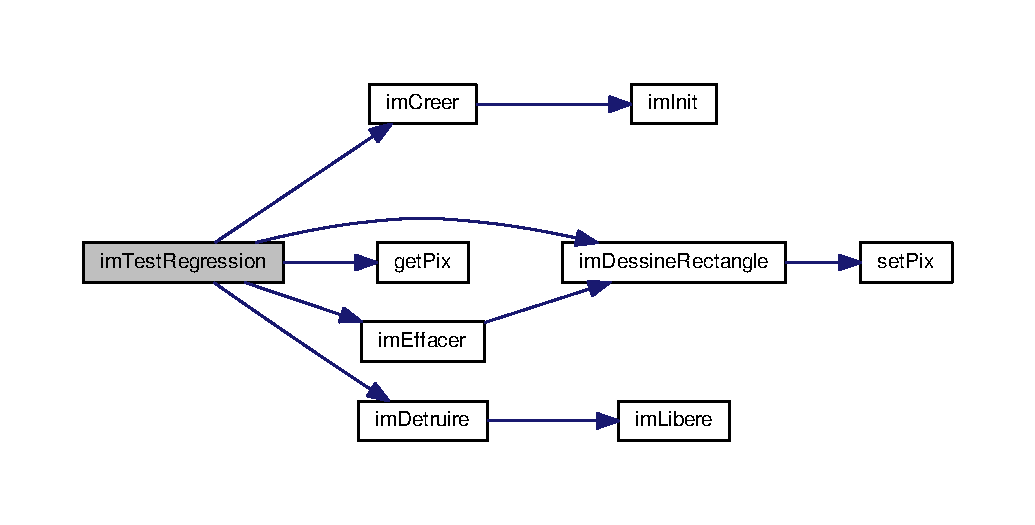
\includegraphics[width=350pt]{Image_8h_a8d4964490fb1a67b590ce77acd78031f_cgraph}
\end{center}
\end{figure}




Here is the caller graph for this function\+:\nopagebreak
\begin{figure}[H]
\begin{center}
\leavevmode
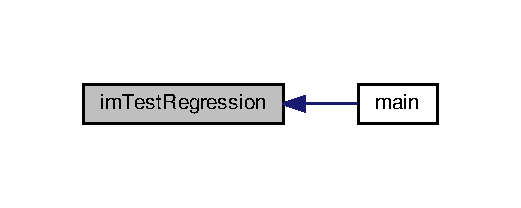
\includegraphics[width=250pt]{Image_8h_a8d4964490fb1a67b590ce77acd78031f_icgraph}
\end{center}
\end{figure}


\hypertarget{Image_8h_a7da553849b645f075994622df5bca888}{}\index{Image.\+h@{Image.\+h}!set\+Pix@{set\+Pix}}
\index{set\+Pix@{set\+Pix}!Image.\+h@{Image.\+h}}
\subsubsection[{set\+Pix}]{\setlength{\rightskip}{0pt plus 5cm}void set\+Pix (
\begin{DoxyParamCaption}
\item[{{\bf Image} $\ast$}]{im, }
\item[{const int}]{x, }
\item[{const int}]{y, }
\item[{{\bf Pixel}}]{couleur}
\end{DoxyParamCaption}
)}\label{Image_8h_a7da553849b645f075994622df5bca888}


set\+Pix modifie le pixel de coordonnées (x,y) 


\begin{DoxyParams}[1]{Parameters}
\mbox{\tt in,out}  & {\em im} & la structure image \\
\hline
\mbox{\tt in}  & {\em x} & Entier qui désigne les cordonnée de l\textquotesingle{}image sur l\textquotesingle{}axe des x \\
\hline
\mbox{\tt in}  & {\em y} & Entier qui désigne les cordonnée de l\textquotesingle{}image sur l\textquotesingle{}axe des y \\
\hline
\end{DoxyParams}
\begin{DoxyReturn}{Returns}
none.
\end{DoxyReturn}

\begin{DoxyCode}
1 setPix(&im,200,352);
\end{DoxyCode}
 \begin{DoxyWarning}{Warning}
x et y doivent etre inclu dans l\textquotesingle{}intervalle des dimensions 
\end{DoxyWarning}


Definition at line 63 of file Image.\+c.


\begin{DoxyCode}
64 \{
65     assert((x<im->dimx) && (y<im->dimy) && (x>=0) & (y>=0));
66 
67     im->\hyperlink{structImage_aad00390430c4e4e3a5a71bb919a4076c}{tab}[x][y]=couleur;
68 
69 
70 \}
\end{DoxyCode}


Here is the caller graph for this function\+:\nopagebreak
\begin{figure}[H]
\begin{center}
\leavevmode
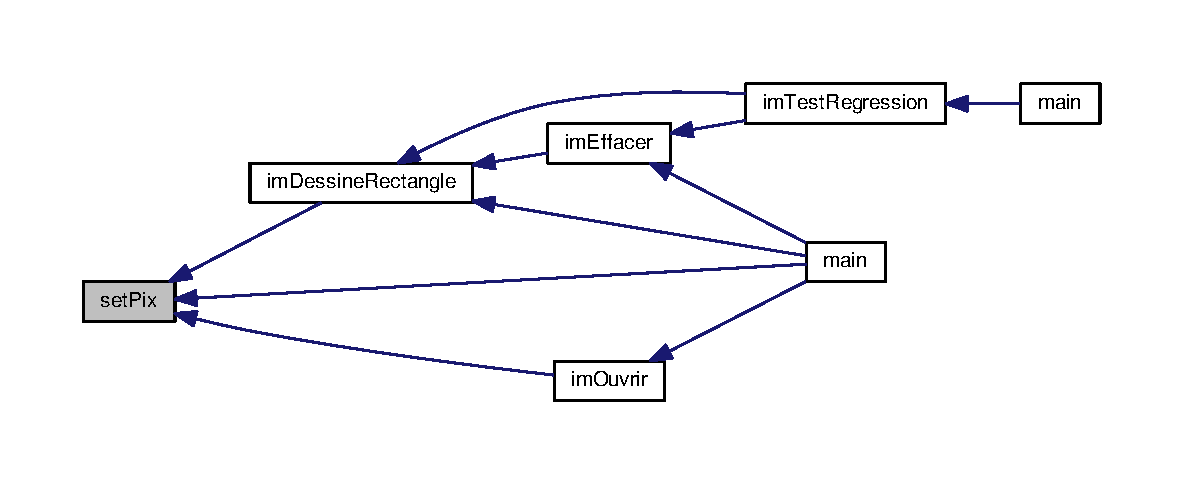
\includegraphics[width=350pt]{Image_8h_a7da553849b645f075994622df5bca888_icgraph}
\end{center}
\end{figure}



\hypertarget{main_8c}{}\section{/home/wadi2a/\+Desktop/11512099/src/main.c File Reference}
\label{main_8c}\index{/home/wadi2a/\+Desktop/11512099/src/main.\+c@{/home/wadi2a/\+Desktop/11512099/src/main.\+c}}


Fichier .c le main du projet Fichier qui comporte le code du projet.  


{\ttfamily \#include $<$stdio.\+h$>$}\\*
{\ttfamily \#include $<$stdlib.\+h$>$}\\*
{\ttfamily \#include \char`\"{}Image.\+h\char`\"{}}\\*
Include dependency graph for main.\+c\+:\nopagebreak
\begin{figure}[H]
\begin{center}
\leavevmode
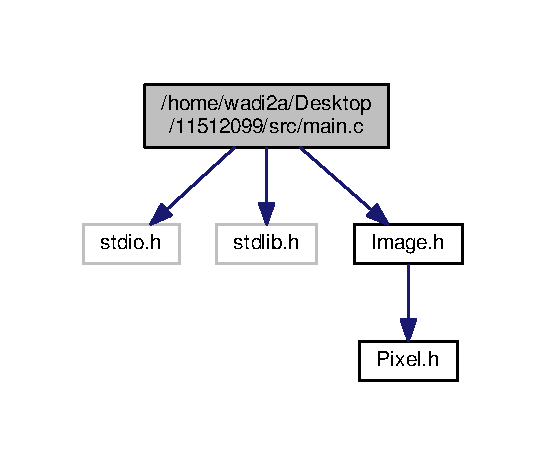
\includegraphics[width=262pt]{main_8c__incl}
\end{center}
\end{figure}
\subsection*{Functions}
\begin{DoxyCompactItemize}
\item 
int \hyperlink{main_8c_ae66f6b31b5ad750f1fe042a706a4e3d4}{main} ()
\end{DoxyCompactItemize}


\subsection{Detailed Description}
Fichier .c le main du projet Fichier qui comporte le code du projet. 

\begin{DoxyAuthor}{Author}
B\+E\+N A\+I\+S\+S\+A O\+U\+A\+D\+I\+E
\end{DoxyAuthor}
\begin{DoxyVersion}{Version}
1.\+0 
\end{DoxyVersion}
\begin{DoxyDate}{Date}
2016/02/10 
\end{DoxyDate}


\subsection{Function Documentation}
\hypertarget{main_8c_ae66f6b31b5ad750f1fe042a706a4e3d4}{}\index{main.\+c@{main.\+c}!main@{main}}
\index{main@{main}!main.\+c@{main.\+c}}
\subsubsection[{main}]{\setlength{\rightskip}{0pt plus 5cm}int main (
\begin{DoxyParamCaption}
{}
\end{DoxyParamCaption}
)}\label{main_8c_ae66f6b31b5ad750f1fe042a706a4e3d4}


Definition at line 25 of file main.\+c.


\begin{DoxyCode}
26 \{
27     
28       \hyperlink{structImage}{Image} im; \hyperlink{structImage}{Image} imb;
29     \hyperlink{structPixel}{Pixel} color = \{ 255, 255, 255 \};
30     \hyperlink{structPixel}{Pixel} color2 = \{ 255, 128, 255 \};
31     \hyperlink{structPixel}{Pixel} color3 = \{ 0, 128, 255 \};
32 
33     \hyperlink{Image_8c_a6edbdf3bfe3beb4e44246a6c7985055c}{imInit}(&im, 500, 500);
34     \hyperlink{Image_8c_ae11c1ca640aae91cb1419158ad5bdf59}{imEffacer}(&im, color);
35 
36     \hyperlink{Image_8c_a01084dc5c10d366999aece5432dc823f}{imDessineRectangle}( &im, 00, 0, 250, 499, color2);
37     \hyperlink{Image_8c_a7da553849b645f075994622df5bca888}{setPix}(&im, 2, 2, color2); \textcolor{comment}{/* change le pixel (2,2) */}
38     \hyperlink{Image_8c_a20b9ad35b6db7bd09d7452574d04dd50}{imSauver}(&im, \textcolor{stringliteral}{"./data/toto.ppm"}); \textcolor{comment}{/* voir section suivante : Debug */}
39 
40     \hyperlink{Image_8c_a0a1f0b9be4b910e1cfc2648cfa9e38fd}{imOuvrir}( &imb, \textcolor{stringliteral}{"./data/toto.ppm"});
41     \hyperlink{Image_8c_a01084dc5c10d366999aece5432dc823f}{imDessineRectangle}( &imb, 5, 5, 15, 10, color3);
42     \hyperlink{Image_8c_a01084dc5c10d366999aece5432dc823f}{imDessineRectangle}( &imb, 25, 25, 35, 45, color3);
43     \hyperlink{Image_8c_a20b9ad35b6db7bd09d7452574d04dd50}{imSauver}( &imb, \textcolor{stringliteral}{"./data/titi.ppm"}); \textcolor{comment}{/* voir section suivante : Debug */}
44 
45     \hyperlink{Image_8c_a5931290abc22d365ae351381c594613f}{imLibere}(&im);
46     \hyperlink{Image_8c_a5931290abc22d365ae351381c594613f}{imLibere}(&imb);
47 
48 \textcolor{keywordflow}{return} 0;
49 \}
\end{DoxyCode}


Here is the call graph for this function\+:\nopagebreak
\begin{figure}[H]
\begin{center}
\leavevmode
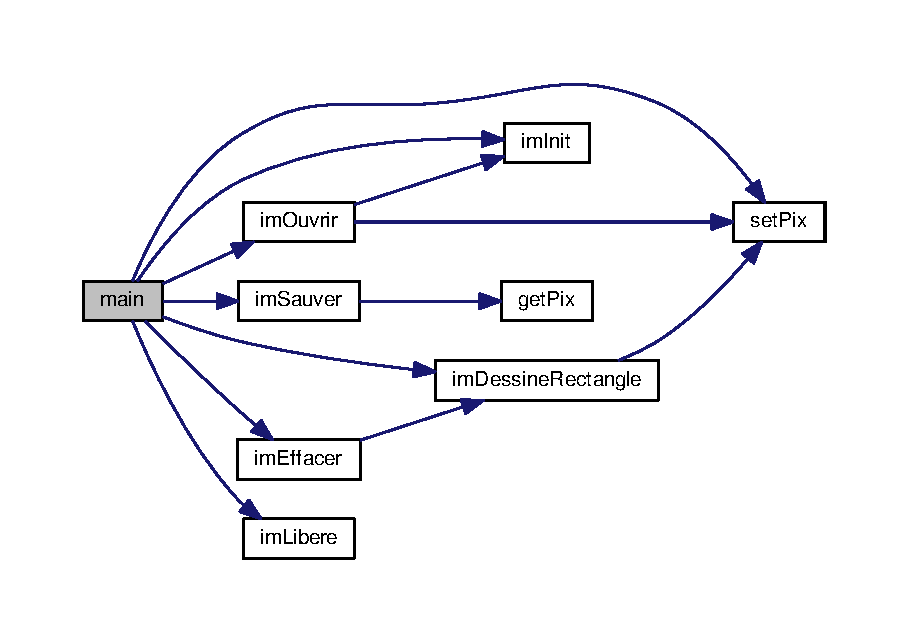
\includegraphics[width=350pt]{main_8c_ae66f6b31b5ad750f1fe042a706a4e3d4_cgraph}
\end{center}
\end{figure}



\hypertarget{mainTest_8c}{}\section{/home/wadi2a/\+Desktop/11512099/src/main\+Test.c File Reference}
\label{mainTest_8c}\index{/home/wadi2a/\+Desktop/11512099/src/main\+Test.\+c@{/home/wadi2a/\+Desktop/11512099/src/main\+Test.\+c}}
{\ttfamily \#include $<$stdio.\+h$>$}\\*
{\ttfamily \#include $<$stdlib.\+h$>$}\\*
{\ttfamily \#include \char`\"{}Image.\+h\char`\"{}}\\*
Include dependency graph for main\+Test.\+c\+:\nopagebreak
\begin{figure}[H]
\begin{center}
\leavevmode
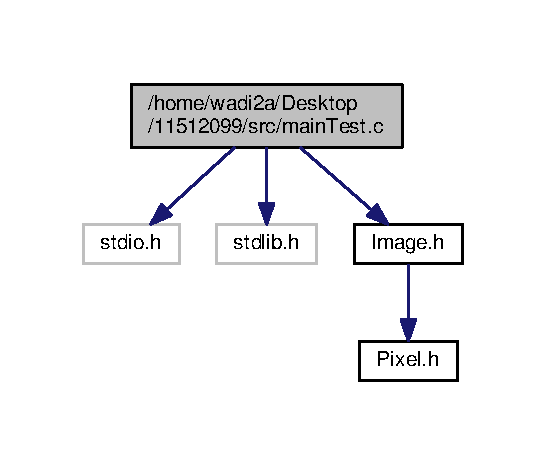
\includegraphics[width=262pt]{mainTest_8c__incl}
\end{center}
\end{figure}
\subsection*{Functions}
\begin{DoxyCompactItemize}
\item 
int \hyperlink{mainTest_8c_ae66f6b31b5ad750f1fe042a706a4e3d4}{main} ()
\end{DoxyCompactItemize}


\subsection{Function Documentation}
\hypertarget{mainTest_8c_ae66f6b31b5ad750f1fe042a706a4e3d4}{}\index{main\+Test.\+c@{main\+Test.\+c}!main@{main}}
\index{main@{main}!main\+Test.\+c@{main\+Test.\+c}}
\subsubsection[{main}]{\setlength{\rightskip}{0pt plus 5cm}int main (
\begin{DoxyParamCaption}
{}
\end{DoxyParamCaption}
)}\label{mainTest_8c_ae66f6b31b5ad750f1fe042a706a4e3d4}


Definition at line 26 of file main\+Test.\+c.


\begin{DoxyCode}
27 \{
28 \hyperlink{Image_8c_a8d4964490fb1a67b590ce77acd78031f}{imTestRegression}();
29 \textcolor{keywordflow}{return} 0;
30 \}
\end{DoxyCode}


Here is the call graph for this function\+:\nopagebreak
\begin{figure}[H]
\begin{center}
\leavevmode
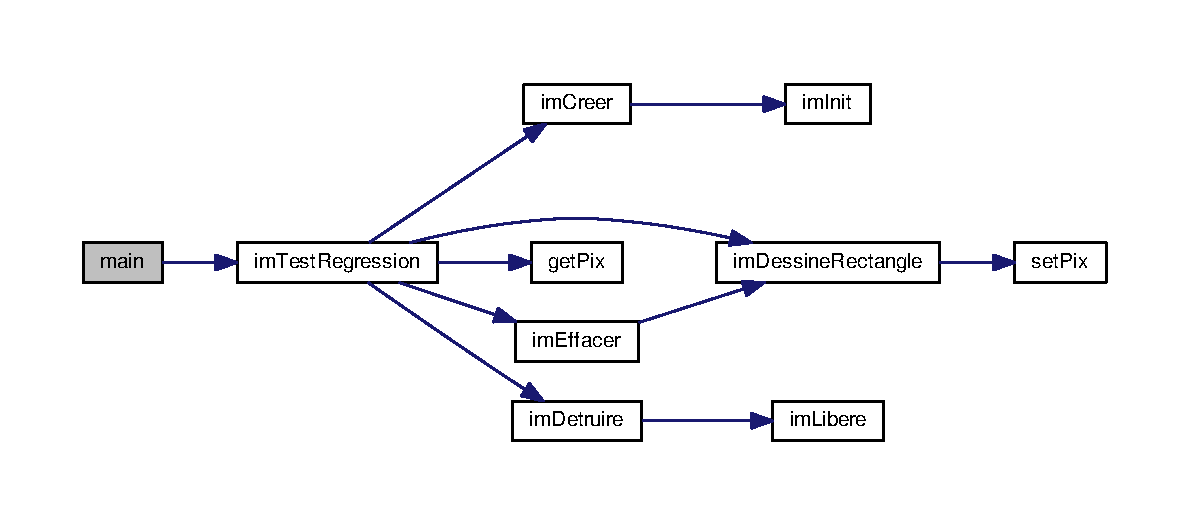
\includegraphics[width=350pt]{mainTest_8c_ae66f6b31b5ad750f1fe042a706a4e3d4_cgraph}
\end{center}
\end{figure}



\hypertarget{Pixel_8c}{}\section{/home/wadi2a/\+Desktop/11512099/src/\+Pixel.c File Reference}
\label{Pixel_8c}\index{/home/wadi2a/\+Desktop/11512099/src/\+Pixel.\+c@{/home/wadi2a/\+Desktop/11512099/src/\+Pixel.\+c}}


Fichier .c du Module \hyperlink{structPixel}{Pixel} Fichier qui comporte tout la définition des fonction de ce module.  


{\ttfamily \#include $<$stdio.\+h$>$}\\*
{\ttfamily \#include $<$stdlib.\+h$>$}\\*
{\ttfamily \#include $<$assert.\+h$>$}\\*
{\ttfamily \#include \char`\"{}Pixel.\+h\char`\"{}}\\*
Include dependency graph for Pixel.\+c\+:\nopagebreak
\begin{figure}[H]
\begin{center}
\leavevmode
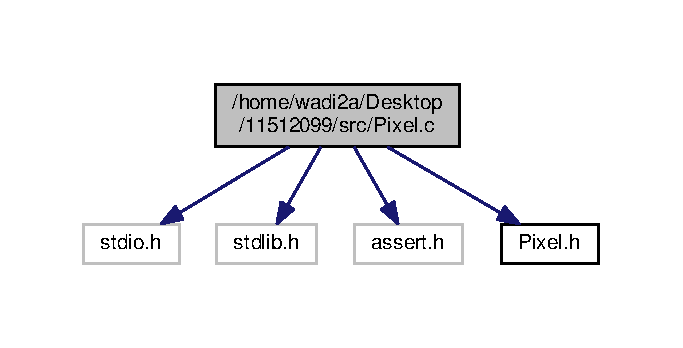
\includegraphics[width=328pt]{Pixel_8c__incl}
\end{center}
\end{figure}


\subsection{Detailed Description}
Fichier .c du Module \hyperlink{structPixel}{Pixel} Fichier qui comporte tout la définition des fonction de ce module. 

\begin{DoxyAuthor}{Author}
B\+E\+N A\+I\+S\+S\+A O\+U\+A\+D\+I\+E
\end{DoxyAuthor}
\begin{DoxyVersion}{Version}
1.\+0 
\end{DoxyVersion}
\begin{DoxyDate}{Date}
2016/02/10 
\end{DoxyDate}

\hypertarget{Pixel_8h}{}\section{/home/wadi2a/\+Desktop/11512099/src/\+Pixel.h File Reference}
\label{Pixel_8h}\index{/home/wadi2a/\+Desktop/11512099/src/\+Pixel.\+h@{/home/wadi2a/\+Desktop/11512099/src/\+Pixel.\+h}}


Fichier .h du Module \hyperlink{structPixel}{Pixel} Fichier qui comporte tout la déclaration des fonctions de ce module.  


This graph shows which files directly or indirectly include this file\+:\nopagebreak
\begin{figure}[H]
\begin{center}
\leavevmode
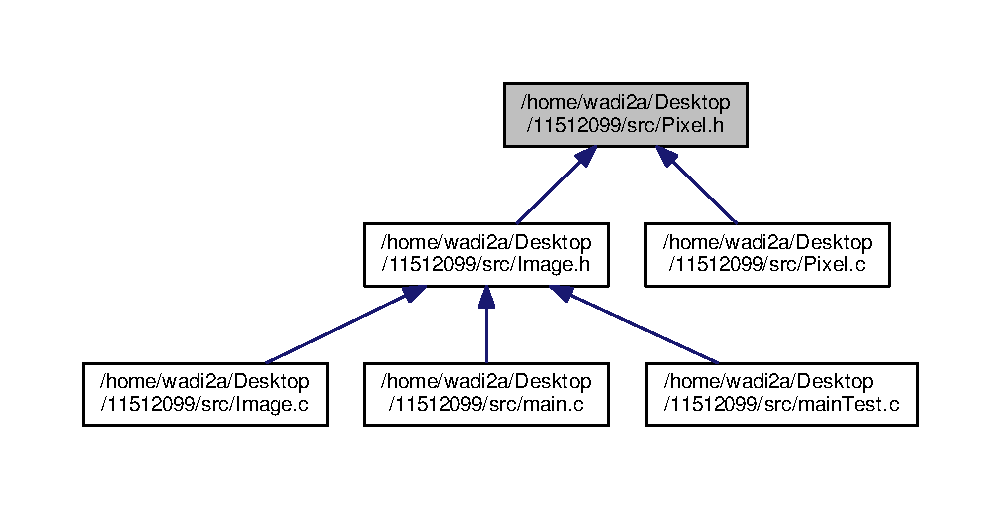
\includegraphics[width=350pt]{Pixel_8h__dep__incl}
\end{center}
\end{figure}
\subsection*{Data Structures}
\begin{DoxyCompactItemize}
\item 
struct \hyperlink{structPixel}{Pixel}
\end{DoxyCompactItemize}
\subsection*{Typedefs}
\begin{DoxyCompactItemize}
\item 
typedef struct \hyperlink{structPixel}{Pixel} \hyperlink{Pixel_8h_adda0c7dd8a357d7d12fe69b89e6dc72a}{Pixel}
\end{DoxyCompactItemize}


\subsection{Detailed Description}
Fichier .h du Module \hyperlink{structPixel}{Pixel} Fichier qui comporte tout la déclaration des fonctions de ce module. 

\begin{DoxyAuthor}{Author}
B\+E\+N A\+I\+S\+S\+A O\+U\+A\+D\+I\+E
\end{DoxyAuthor}
\begin{DoxyVersion}{Version}
1.\+0 
\end{DoxyVersion}
\begin{DoxyDate}{Date}
2016/02/10 
\end{DoxyDate}


\subsection{Typedef Documentation}
\hypertarget{Pixel_8h_adda0c7dd8a357d7d12fe69b89e6dc72a}{}\index{Pixel.\+h@{Pixel.\+h}!Pixel@{Pixel}}
\index{Pixel@{Pixel}!Pixel.\+h@{Pixel.\+h}}
\subsubsection[{Pixel}]{\setlength{\rightskip}{0pt plus 5cm}typedef struct {\bf Pixel} {\bf Pixel}}\label{Pixel_8h_adda0c7dd8a357d7d12fe69b89e6dc72a}


Definition at line 18 of file Pixel.\+h.


%--- End generated contents ---

% Index
\backmatter
\newpage
\phantomsection
\clearemptydoublepage
\addcontentsline{toc}{chapter}{Index}
\printindex

\end{document}
